\ifnum\switch=1
% -----------------------------------------------------------------------------
% ------------------------------ Extended ToC ---------------------------------
% -----------------------------------------------------------------------------
%data mostly gotten from: PHD_Docs/LaTeX/Shishkin/ETNA17001_revised/Ech.Lie.Szy.Tic.17_rev.tex
Parts of this chapter have already been published in:
\begin{enumerate}
\item[\cite{EchLieSzyTic18}] \underline{C.~Echeverr{\'\i}a}, J.~Liesen, D.~B.~Szyld, and P.~Tich{\'y}, \textbf{Convergence of the multiplicative Schwarz method for singularly perturbed convection-diffusion problems discretized on a Shishkin mesh}, Electron. Trans. Numer. Anal., 48 (2018), pp. 40--62.
\end{enumerate}


\section{Introduction}
This section is based on the following references: \cite{EchLieSzyTic18, GriDolSil15}.
\paragraph{Keywords:} Bounds on Infinity norm, solving linear systems with mSm,


\section{The Model Problem and its Shishkin Mesh Discretization}
This section is based on the following references: \cite{GriDolSil15, Lin10, RooStyTob08, Sty05}.


\section{Convergence Bounds for the Multiplicative Schwarz Method}
This section is based on the following reference: \cite{EchLieSzyTic18}.


\subsection{Bounds for the Upwind Difference Scheme}


\subsection{Bounds for the Central Difference Scheme}


\section{The Stagnation of GMRES}
This section is based on the following references: \cite{Gal13, GolVan13, HorJoh12, Saa03}.
\paragraph{Keywords:} Eigenvalue analysis is useless


\section{Shishkin-Schwarz Preconditioning}
This section is based on the following references: \cite{EchLieSzyTic18, KahKamPhi07}.


\section{Flow-Following Preconditioning}
This section is based on the following references: \cite{EchGarSet19, ElmSilWat14}.
\paragraph{Keywords:} The name flow following comes from \cite{AndKop96}


\section{Numerical Experiments}
This section is based on the following references: \cite{ElmSilWat14}.

\subsection{Upwind Finite Differences}
This section is based on the following references: \cite{EchLieSzyTic18, Smi85}.


\subsection{Central Finite Differences}
This section is based on the following references: \cite{EchLieSzyTic18, Smi85}.


\else
% -----------------------------------------------------------------------------
% --------------------------- Content of Chapter ------------------------------
% -----------------------------------------------------------------------------

Parts of this chapter have already been published in:
\vspace*{0.3cm}
%
\begin{enumerate}
\item[\cite{EchLieSzyTic18}] \underline{C.~Echeverr{\'\i}a}, J.~Liesen, D.~B.~Szyld, and P.~Tich{\'y}, \textbf{Convergence of the multiplicative Schwarz method for singularly perturbed convection-diffusion problems discretized on a Shishkin mesh}, Electron. Trans. Numer. Anal., 48 (2018), pp. 40--62.
\end{enumerate}
%
\vspace*{0.25cm}
%
\section{Introduction}
\label{1D:intro}

In this chapter we study the convergence behavior of the multiplicative
Schwarz method when it is used to solve linear systems of the form
%
\begin{equation}\label{eq:1D:linsys}
\mathbf{A}\mathbf{u}=\mathbf{f},
\end{equation}
%
where the coefficient matrix is obtained from finite difference discretizations
of the following one-dimensional constant coefficient convection-diffusion BVP
with Dirichlet boundary conditions posed on a Shishkin mesh:
\begin{equation}\label{eq:1D:bvp}
\begin{cases}
%-\epsilon  u''(x) + \omega u'(x)+\beta u(x) = f(x), & \text{in}\; (0,1)\\
-\epsilon\frac{\partial^2 u(x)}{\partial x^2}+\omega_x \frac{\partial u(x)}{\partial x} + \beta u(x)=f(x), & \text{in}\; (0,1)\\
\hspace{0.8cm} u(0)=g_0,\;\text{ and }\;u(1)=g_1, &
\end{cases}
% \begin{cases}
% %\mathscr{A}u(x)\equiv
% -\epsilon  u''(x) + \omega_x u'(x)+\beta u(x) = f(x), &  0<x<1,\\
%             \qquad\;\;u(0)=g_0,\;\;u(1)=g_1. &
% \end{cases}
\end{equation}
%
We assume $\omega_x\gg \epsilon >0$ and $\beta\geq 0$ and that the parameters
of the problem, i.e., $\epsilon,\omega_x,\beta,f,g_0,$ and $g_1$, are chosen
so that the solution $u(x)$ has one boundary layer close to the point $x=1$.
We resolve the boundary layer using a finite difference discretization on a
one-dimensional Shishkin mesh with transition point close to $x=1$ and
consider two different schemes on the mesh: upwind and central differences.

After the discretization process, the structure of the coefficient matrix,
$\A$ in \eqref{eq:1D:linsys}, takes the form:
%
\begin{equation}\label{eq:1D:struct}
\A=\left[
  \begin{array}{c|c|c}
     \matAH & \entryvE &          \\ \hline
  \entryzW  & \entryzC & \entryzE \\ \hline
            & \entrywW & \matAh
  \end{array}
\right],%\;\in\;{\mathbb R}^{(N-1)\times (N-1)}.
\end{equation}
where the matrices $\matAH$ and $\matAh$ %\;\in\;{\mathbb R}^{(n-1)\times (n-1)}$
are given by:
\begin{equation}
\matAH = \text{tridiag}(\entryvW, \entryvC, \entryvE),\quad \text{and} \quad
\matAh = \text{tridiag}(\entrywW, \entrywC, \entrywE),
\end{equation}
%
and $\entryvW, \entryvC, \entryvE,\entrywW, \entrywC, \entrywE\in\Re$. In turn,
the structure of the coefficient matrix \eqref{eq:1D:struct} induces a very
special rank-one structure of the iteration matrices $\T_{ij}$, defined in
\eqref{eq:back:Tij} and used in the multiplicative Schwarz method. Using the
resulting algebraic structure of the iteration matrices, we derive bounds on
the infinity norm of the error produced by the method at each iteration step.
Unlike asymptotic convergence results based on bounding the spectral radius of
the iteration matrix, our results apply to the transient rather than the
asymptotic behavior and thus our error bounds are valid from the first step of
the multiplicative Schwarz iterations.

For linear systems obtained from the upwind scheme we prove rapid convergence
of the  multiplicative Schwarz iteration for all relevant parameters in the
problem. The analysis of the central difference scheme is more complicated,
since some of the submatrices that occur in this case are not only
nonsymmetric, but also fail to be $M$-matrices. This reminds of the analysis
in~\cite{AndKop96}, which showed that in this case the difference scheme
itself does not satisfy a discrete maximum principle. Nevertheless, we can
prove the convergence of the multiplicative Schwarz method for problems
discretized by central differences on a Shishkin mesh under the assumption
that the number of discretization points in each of the local subdomains is
even. If this assumption is not satisfied, then the method may diverge, which
we also explain in our analysis.

Furthermore, we study the convergence of the preconditioned GMRES method when
the multiplicatvie Schwarz method is used as a preconditioner and show that the
low-rank structure of the iteration matrices $\T_{ij}$ is enough to prove
convergence of the preconditioned GMRES method independently of the
perturbation parameter~$\epsilon$.
%We also present the ideas of \emph{Flow-Following} preconditioners and provide an analysis of convergence of GMRES when these type of preconditioning is used and show that they are efficient in getting rid of the well-known stagnation of GMRES (see \cite{LieStr03}) present when used to solve linear systems with the
%unpreconditioned system.

The chapter is organized as follows. We immediately begin by presenting
the convergence analysis of the multiplicative Schwarz method in
Section~\ref{1D:bounds}; first for the upwind scheme and
then for the central difference scheme. Background material including the
Shishkin mesh discretization of the one-dimensional model problem is specified
in previous chapters (see Chapter~\ref{ch:back}). In Section~\ref{1D:ShishScwarzPrecon} we discuss the performance of GMRES when
preconditioned with the multiplicative Schwarz method.
%In Section~\ref{1D:FlowFollowPrecon} we present an analysis of the convergence
%of GMRES when a second type of preconditioners, \emph{Flow-Following preconditioners}, are used.
Numerical examples are shown in Section~\ref{1D:NumericsA}.

%\hfill
%\newpage

% \section{The Shishkin Mesh Discretization of the Model Problem}
% \label{1D:ModProb}
%
% We consider the one-dimensional convection-diffusion boundary value
% problem with constant coefficients and Dirichlet boundary conditions given by
% \eqref{eq:1D:bvp} and proceed to apply the finite difference procedure
% described in Section \ref{back:convdiff:findiff} on the one-dimensional
% Shishkin mesh presented in Section \ref{back:convdiff:shihs1D} and shown in
% Figure \ref{fig:back:shmesh1D}.
%
% % The first derivative of $u$ at the point $x_i$ approximated by the standard
% % upwind finite difference operator (see Section \ref{back:convdiff:findiff}) is
% % given by
% % \begin{equation*}
% % %\frac{\partial u(x_i)}{\partial x}
% % u'(x_i)\approx
% % %(\Delta x)^{-1}D^{-}_{x} u_{i}^D = (\Delta x)^{-1}(u_{i}^D-u_{i-1}^{N})=
% % \frac{u_i^D-u_{i-1}^{N}}{h_i},
% % \end{equation*}
% % and using the central finite difference operator we obtain
% % \begin{equation*}\label{eq:firstcen}
% % %\frac{\partial u(x_i)}{\partial x}
% % u'(x_i)\approx %(\Delta x)^{-1} D^{0}_{x} u_{i}^D =(\Delta x)^{-1}(u_{i+1}^D-u_{i-1}^{N})=
% % \frac{u_{i+1}^D-u_{i-1}^{N}}{(h_i+h_{i+1})}.
% % \end{equation*}
% % The second derivative can be approximated by
% % \begin{equation*}
% % %\frac{\partial u(x_i)}{\partial x^2}
% % u''(x_i)\approx %\delta^{2}_{x} u_{i}^D\; =\;
% % \frac{2 u_{i-1}^D}{(h_{i} + h_{i+1}) h_{i+1}}- \frac{2u_{i}^D}{h_{i} h_{i+1}} + \frac{2 u_{i+1}^D}{(h_{i} + h_{i+1}) h_{i+1}}.
% % \end{equation*}
% Applying the discrete operators given in Table~\ref{tab:back:findiff} on the
% nodes of the Shishkin mesh, where $h_i=H_x$ for $i=1,\ldots,n$ and $h_i=h_{x}$
% for $i=n+1,\ldots,N-1$, we obtain for the upwind scheme:
% \begin{equation}
% \Delta^{-}_{x} u_{i}^D\; =\;
% \begin{cases}
% \frac{1}{H_x}\left(u_{i}^D-u_{i-1}^D\right) & \mbox{for}\;\; i=1,\ldots, n, \\
% \frac{1}{h_x}\left(u_{i}^D-u_{i-1}^D\right) & \mbox{for}\;\; i={n+1},\ldots, N-1,
% \end{cases}
% \end{equation}
% and for the central finite difference scheme we obtain
% \begin{equation}
% \Delta^{0}_{x} u_{i}^D\; =\;
% \begin{cases}
% \frac{1}{2H_x}\left(u_{i+1}^D-u_{i-1}^D\right) &
% \mbox{for}\;\; i=1,\ldots, {n-1},\\
% \frac{1}{h_x+H_x}\left(u_{i+1}^D-u_{i-1}^D\right)  &
% \mbox{for}\;\; i=n,\\
% \frac{1}{2h_x}\left(u_{i+1}^D-u_{i-1}^D\right)  &
% \mbox{for}\;\;i={n+1},\ldots, {N-1}.
% \end{cases}
% \end{equation}
% For the second derivatives, we obtain
% \begin{equation}\label{eq:back:second}
% \delta^{2}_{x} u_{i}^D\; =\;
% \begin{cases}
% \frac{1}{H_x^2}\left(u_{i-1}^D - 2u_{i}^D + u_{i+1}^D\right) &
% \mbox{for}\;\; i=1,\ldots, {n-1},\\
% \frac{2u_{i-1}^D}{(H_x+h_x)H_x} - \frac{2u_{i}^D}{H_xh_x} + \frac{2u_{i+1}^D}{(H_x+h_x)h_x} &
% \mbox{for}\;\; i=n,\\
% \frac{1}{h_x^2}\left(u_{i-1}^D - 2u_{i}^D + u_{i+1}^D\right) &
% \mbox{for}\;\;i={n+1},\ldots, {N-1}.
% \end{cases}
% \end{equation}
%
% % Considering the homogeneous boundary conditions $u_0 = u_1 = 0$ and letting
% % $\omega(x)=\omega>0$, and $\beta(x) = \beta>0$ be constant along the domain,
% % the finite difference scheme applied to the differential equation in \eqref{eq:1D:bvp} on
% % the Shishkin mesh is then given~by
% % \begin{equation}\label{eq:1DdiscrOp}
% % %\Au^D_m\equiv
% % -\epsilon \delta_x^2 u^D_i + \omega \Delta^{-/0}_{x}u^D_i +\beta_i u^D_i= f_i,\quad i=1,2,\ldots,N-1\equiv M.
% % \end{equation}
% Thus, by including the boundary conditions and letting $\omega(x)=\omega_x>0$
% and $\beta(x) = \beta > 0$ be constant along the domain, the finite difference
% scheme applied to the continuous problem \eqref{eq:1D:bvp} results in the
% discrete version of our model problem:
% % consists of the
% % following discretization of the one-dimensional convection-diffusion boundary
% % value problem with constant coefficients and Dirichlet boundary conditions:
% %
% \begin{equation}\label{eq:back:1DbvpDiscr}
% \begin{cases}
% %\A\u\equiv
% -\epsilon \delta^2 u^D_i + \omega_i \Delta^{-/0}u^D_i +\beta_i u^D_i = f_i, & i=1,\ldots,N-1,\\
% \;\;u^D_0=g_0,\;\;u^D_N=g_1, &
% \end{cases}
% \end{equation}
%
% By collecting all equations for $i=1,\ldots,N-1$, both finite difference schemes
% yield a linear algebraic system \eqref{eq:1D:linsys} with the tridiagonal and
% nonsymmetric $(N-1)\times (N-1)$ coefficient matrix given by:
% %
% \begin{equation}\label{eq:back:1Dmatrix}
% \A=\left[
%   \begin{array}{cccc|c|cccc}
%      \entryvC &\entryvE    &  &  &  &  &  &  &  \\
%      \entryvW &\ddots &\ddots  &  &  &  &  &  &  \\
%      &  \ddots& \ddots &  \entryvE   &  &  &  &  &  \\
%      &  &\entryvW & \entryvC  & \entryvE   &  &  &  &  \\ \hline
%      &  &  & \entryzW  & \entryzC  & \entryzE  &  &  &  \\ \hline
%      &  &  &  & \entrywW  & \entrywC  & \entrywE  &  &  \\
%      &  &  &  &  & \entrywW  & \ddots & \ddots &  \\
%      &  &  &  &  &  & \ddots & \ddots & \entrywE  \\
%      &  &  &  &  &  &  & \entrywW  & \entrywC  \\
%   \end{array}
% \right].%\;\in\;{\mathbb R}^{(N-1)\times (N-1)}.
% \end{equation}
% %
% For the upwind scheme, the entries of $\A$ are given by
% %
% \begin{align}
%     &\entryvW  =  -\frac{\epsilon}{H^{2}} - \frac{\omega_x}{H},&
%     &\entryvC  =  \frac{2\epsilon}{H^{2}} + \frac{\omega_x}{H}+\beta, &
%     &\entryvE   =  -\frac{\epsilon}{H^{2}}, \nonumber \\
%     &\entryzW  =  -\frac{2\epsilon}{H(H+h)} - \frac{\omega_x}{H},&
%     &\entryzC  =  \frac{2\epsilon}{hH} + \frac{\omega_x}{H}+\beta,&
%     &\entryzE  =  -\frac{2\epsilon}{h(H+h)}, \label{eq:back:upwind} \\
%     &\entrywW  =  -\frac{\epsilon}{h^{2}} - \frac{\omega_x}{h},&
%     &\entrywC  =  \frac{2\epsilon}{h^{2}} + \frac{\omega_x}{h}+\beta,&
%     &\entrywE  =  -\frac{\epsilon}{h^{2}}, \nonumber
% \end{align}
% %
% and for the central difference scheme by
% %
% \begin{align}
%     &\entryvW  =  -\frac{\epsilon}{H^{2}} - \frac{\omega_x}{2H},&
%     &\entryvC  =  \frac{2\epsilon}{H^{2}} + \beta, &
%     &\entryvE  =  -\frac{\epsilon}{H^{2}}+\frac{\omega_x}{2H}, \nonumber \\
%     &\entryzW  =  -\frac{2\epsilon}{H(H+h)} -\frac{\omega_x}{h+H},&
%     &\entryzC  =  \frac{2\epsilon}{hH} + \beta,&
%     &\entryzE  =  -\frac{2\epsilon}{h(H+h)}+\frac{\omega_x}{h+H}, \label{eq:back:central} \\
%     &\entrywW  =  -\frac{\epsilon}{h^{2}} - \frac{\omega_x}{2h},&
%     &\entrywC  =  \frac{2\epsilon}{h^{2}} +\beta,&
%     &\entrywE  =  -\frac{\epsilon}{h^{2}}+ \frac{\omega_x}{2h}. \nonumber
% \end{align}
%
% % Moreover, we can express the system matrix \eqref{eq:back:1Dmatrix} using the
% % standard finite difference matrices, see,~\cite[Section~2]{PalSim15}. Consider
% % the following proposition:
% % %
% % \begin{prop}
% % Let $x_i\in\Omega^D=\{x_i\in\overline{\Omega}:i=0,\ldots,N;\},$
% % be the $N+1$ nodes of the Shishkin mesh. Then the upwind finite
% % difference discretization of the differential operator in \eqref{eq:1D:bvp}
% % leads to the following discrete operator:
% % \begin{equation}\label{eq:1Dkronrep}
% % A =
% % \epsilon (D_{xx}T+e_{n}v_{x}^T) + \omega_xD_xB_{up/cd} + \beta I,
% % \end{equation}
% % where
% % \begin{eqnarray}
% % T      &=& \mathrm{tridiag}(1,-2,1) \in \mathbb{R}^{M\times M},\nonumber\\
% % B_{up} &=& \mathrm{tridiag}(-1,1,0) \in \mathbb{R}^{M\times M},\nonumber\\
% % B_{cd} &=& \mathrm{tridiag}(-1,1,-1)\in \mathbb{R}^{M\times M},\nonumber\\
% % D_{x}  &=& \mathrm{diag}\left(\underbrace{H_x^{-1},\dots,
% %            H_x^{-1}}_{n},\underbrace{h_x^{-1},\ldots,
% %            h_x^{-1}}_{m}\right)\in\mathbb{R}^{M\times M},\\
% % D_{xx} &=& \mathrm{diag}\left(\underbrace{-H_x^{-2}, \ldots, -H_x^{-2}}_{m},
% %            -H_x^{-1}h_x^{-1}, \underbrace{-h_x^{-2},\ldots, -h_x^{-2}}_{m}
% %            \right)\in\mathbb{R}^{M\times M},\nonumber \\
% % \omega_x &=& \mathrm{diag}(\omega(x_1),\ldots,
% %              \omega(x_{N-1}))\in\mathbb{R}^{M\times M},\nonumber \\
% % v_x  &=& [\underbrace{0,\ldots,0}_{m-1},-\gamma_x,0,\gamma_x,\underbrace{0,\ldots,0}_{m-1}]^T\in\mathbb{R}^{M\times 1},\nonumber
% % %\quad \gamma_y&=\frac{h_y-H_y}{(H_y+h_y)H_yh_y},\nonumber\\
% % \end{eqnarray}
% % with $\gamma_x=\frac{h_x-H_x}{(H_x+h_x)H_xh_x}$ and $e_n$ is the $n$-th
% % cannonical vector of $\mathbb{R}^{N-1}$.
% % \end{prop}
% %
% % \begin{proof}
% % From\td{\textbf{note}: this proof is for the 2D case, adapt to the 1D case.} \eqref{eq:back:second}
% % we have that, on the Shishkin mesh, the second derivative in the $x$-direction
% % can be approximated by
% % \begin{equation*}\label{eq:secondx}
% % \hspace*{-2em}\delta^{2}_{x} u_{C}\; =\;
% % \frac{1}{H_x^2}\left[1,-2,1\right]\left[\begin{array}{c} u_W\\u_C\\u_E\end{array}\right] \mbox{for}\;\; i=1,\ldots, K,
% % \end{equation*}
% % while the second derivative in the $y$-direction (on the Shishkin mesh) can be
% % approximated by
% % \begin{equation*}\label{eq:secondy}
% % \hspace*{-2em}\delta^{2}_{y} u_{C}\; =\;
% % \begin{cases} \left[u_S,u_C,u_N\right]\frac{1}{H_y^2}\left[\begin{array}{c} 1\\-2\\1\end{array}\right] &\mbox{for}\;\; i=1,\ldots, m, \\
% % \left[u_S,u_C,u_N\right]\frac{1}{H_yh_y}\left[\begin{array}{c} 1\\-2\\1\end{array}\right] + \left[u_S,u_C,u_N\right]\left[\begin{array}{c}\frac{h_y-H_y}{(H_y+h_y)H_yh_y} \\0\\\frac{H_y-h_y}{(H_y+h_y)H_yh_y}\end{array}\right] &\mbox{for}\;\; i=n,\\
% % \left[u_S,u_C,u_N\right]\frac{1}{h_y^2}\left[\begin{array}{c} 1\\-2\\1\end{array}\right] &\mbox{for}\;\; i=n+1,\ldots, M.\end{cases}
% % \end{equation*}
% % Collecting these relations for all rows $i$ and for all columns $j$ for the
% % whole domain we obtain
% % \[
% % -\frac{\partial^2 u(x_i,y_j)}{\partial x^2}\approx D_{xx}TU,\quad -\frac{\partial^2 u(x_i,y_j)}{\partial y^2}\approx U(D_{yy}T+v_ye_n^T),
% % \]
% % with $D_{xx}$, $D_{yy}$, $v_x$ and $v_y$ defined as above.  The matrix $T$
% % represents the unscaled approximations to the second derivative in one
% % dimension. The matrices $D_{xx}$ and $D_{yy}$ are the scaling matrices which
% % account for the different mesh sizes of the hybrid mesh in each direction. The
% % term $e_nv_y^T$ is a rank-one operator which, when added to the scaled matrix,
% % accounts for the uneven factor which multiplies the middle point $y_n$ in the
% % $y$-direction of the mesh. With these approximations we can write the following
% % classical matrix formulation of the finite difference discretization of the
% % Poisson equation on a square domain discretized by a hybrid mesh
% % %
% % \begin{equation}\label{eq:PoissonMatrix}
% % D_{xx}TU+ U(D_{yy}T+v_ye_n^T)=F,\quad\text{where}\quad F_{i,j}=f(x_i,y_j) + \text{b.c.}
% % \end{equation}
% % We can now reshape this matrix equation to obtain its Kronecker formulation;
% % see \cite[Section 1.3.7]{GolVan13}. We know that for a matrix equation $Y=CXB$,
% % where $X$ is the matrix of unknowns, it holds that
% % \[ \text{vec}(Y)=\text{vec}(CXB)=(B^T\otimes C)\text{vec}(X).\]
% % By applying this result to \eqref{eq:PoissonMatrix} we obtain the following
% % formulation,
% %  \begin{equation}\label{eq:PoissonKron}
% %  (I_M\otimes T_x + T_y\otimes I_M+e_nv_y^T \otimes I_M)\text{vec}(U)=\text{vec}(F),
% %  \end{equation}
% % with $T_x=D_{xx}T$, and $T_y=D_{yy}T$. Thus, the discrete Laplacian on the
% % hybrid mesh is
% %  \begin{equation}\label{eq:PoissonKron}
% % I_M\otimes T_x +(T_y+ e_nv_y^T) \otimes I_M.
% %  \end{equation}
% % It remains to show the Kronecker structure of the first order term of \eqref{eq:bvp}.
% %
% % When we assume separable convection coefficients, we have
% % \begin{align*}
% % \omega_x \cdot \nabla u &=(\phi_1(x_i)\psi_1(y_j),\phi_2(x_i),\psi_2(y_j))\cdot\left( \frac{\partial u(x_i,y_j)}{\partial x},\frac{\partial u(x_i,y_j)}{\partial y}\right)\\
% % &\approx \phi_1(x_i)\psi_1(y_j)D^{-}_{x} u_{C} + \phi_2(x_i)\psi_2(y_j)D^{-}_{y} u_{C}.
% % \end{align*}
% % We can approximate these terms by using \eqref{eq:firstup}; for the $x$-
% % direction we obtain
% % \begin{equation*}
% % \phi_1(x_i)\psi_1(y_j)D^{-}_{x} u_{C}\; =\;
% % \frac{1}{H_x}\phi_1(x_i)\left[-1,1,0\right]\left[\begin{array}{c} u_W\\u_C\\u_E\end{array}\right]\psi_1(y_j) \mbox{for}\;\; i=1,\ldots, K.
% % \end{equation*}
% % For the $y$-direction (from the right) we obtain
% % \begin{equation*}
% % \hspace*{-1em}\phi_2(x_i)\psi_2(y_j)D^{-}_{y} u_{C}\; =\;
% % \begin{cases} \phi_2(x_i)\frac{1}{H_y}\left[u_S,u_C,u_N\right]\left[\begin{array}{c} -1\\1\\0\end{array}\right]\psi_2(y_j) &\mbox{for}\;\; i=1,\ldots, n, \\
% %  \phi_2(x_i)\frac{1}{h_y}\left[u_S,u_C,u_N\right]\left[\begin{array}{c} -1\\1\\0\end{array}\right]\psi_2(y_j)&\mbox{for}\;\; i=n+1,\ldots, M.\end{cases}
% % \end{equation*}
% % Collecting these results for all grid nodes and recalling that $u_C$ is the
% % approximation of $u$ at the point $(x_i,y_j)$, we obtain
% % \begin{eqnarray*}
% % \left(\phi_1(x_i)\psi_1(y_j)\frac{\partial u(x_i,y_j)}{\partial x}\right)_{i,j=0,\ldots,J}\approx\Phi_{1}(D_xBU)\Psi_{1},\\
% % \left(\phi_2(x_i)\psi_2(y_j)\frac{\partial u(x_i,y_j)}{\partial y}\right)_{i,j=0,\ldots,N}\approx\Phi_{2}U(D_yB)^T\Psi_{2}.
% % \end{eqnarray*}
% % Thus \eqref{eq:bvp} has the following matrix equation representation
% % \begin{equation*}
% % \epsilon D_{xx}TU + \epsilon U(D_{yy}T+e_nv_y^T) +\Phi_{1}(D_xB)U\Psi_{1}+\Phi_{2}U(D_yB)^T\Psi_{2}=F,
% % \end{equation*}
% % or, equivalently, by applying \cite[Lemma~6.5]{Dem97} we obtain its Kronecker
% % formulation:
% % \[
% % \hspace*{-2em}
% %  \left[\epsilon \left(I_M\otimes T_x\right) +\epsilon\left(T_y\otimes I_M+t_y \otimes I_M\right) + \Psi_1 \otimes \Phi_1B_{x} + \Psi_2B_{y} \otimes \Phi_2\right]\text{vec}(U) =\text{vec}(F).
% % \]
% % Thus we have shown that the discrete operator takes the desired form
% % \eqref{eq:1Dkronrep}.
% % \end{proof}
%
% If $\u=\A^{-1}\f=[u_1^D,\dots,u_{N-1}^D]^T$ is the exact algebraic
% solution, and $u(x)$ is the solution of \eqref{eq:1D:bvp}, then there exist
% constants $c_1,c_2>0$ such that
% %
% $$\max_{1\leq i\leq N-1}\,|u(x_i)-u_i^D| \leq c_1 \frac{\ln N}{N}$$
% %
% for the upwind scheme, and
% %
% $$\max_{1\leq i\leq N-1}\,|u(x_i)-u_i^D| \leq c_2 \left(\frac{\ln N}{N}\right)^2$$
% %
% for the central difference scheme. Thus, the convergence of both schemes is
% $\epsilon$-uniform, and the central difference scheme is more accurate than the
% upwind scheme. As pointed out by Stynes~\cite[p.~470]{Sty05}, the convergence
% proof for the central differences (originally due to Andreyev and
% Kopteva~\cite{AndKop96}) is complicated since the scheme does not satisfy a
% discrete maximum principle. We meet similar complications in our analysis in
% Section~\ref{1D:SchBnds:central} below.



\section{Convergence Bounds for the Multiplicative Schwarz Method}\label{1D:bounds}

As mentioned in Section \ref{back:convdiff:shihs1D}, in this simple
one-dimensional case, the Shishkin mesh divides the discretized domain into two
local subdomains where the solution presents a different characteristic nature.
Therefore, a solution approach based on domain decomposition methods seemed
only natural. For the upwind scheme, we proved rapid convergence of the
multiplicative Schwarz method for all relevant problem parameters. The
convergence for the central difference scheme is slower, but still rapid, when
$N^2\epsilon < \omega_x$ and if $N/2-1$ is even.

\subsection{Structure of the iteration matrices}
\label{1D:bounds:structure}

We start with a closer look at the structure of the iteration matrices
$\T_{ij}$. Note that the matrices $\P_i$ from \eqref{eq:back:Pi} satisfy
%
\begin{equation}\label{eq:1D:P1struct}
\P_1 = \R_1^{\Tr}\R_1\A
=\left[\begin{array}{c} \I_{n}\\ 0\end{array}\right]\A_1^{-1}
\left[\begin{array}{c|c|c}\A_1^{-1} & \entryzE \e_n & 0\end{array}\right]=
\left[\begin{array}{c|c|c}\I_{n}&\entryzE \A_1^{-1}\e_{n}&0\\\hline 0&0&0\end{array}\right],
\end{equation}
%
and
%
\begin{equation}\label{eq:1D:P2struct}
\P_2 = \R_2^{\Tr}\A_2^{-1}\R_2\A =
\left[\begin{array}{c} 0 \\  \I_n\end{array}\right] \A_2^{-1}
\left[\begin{array}{c|c|c}0 & \entryzW \e_1 & \A_2^{-1} \end{array}\right]=
\left[\begin{array}{c|c|c}0&0&0\\\hline0&\entryzW \A_2^{-1}\e_1 & \I_{n}\end{array}\right],
\end{equation}
%
where $\e_1$, $\e_n\in \mathbb{R}^n$. We now denote
%
\begin{equation}\label{eq:1D:p_and_pi}
\left[\begin{array}{c}\pOne \\\hline \piOne\end{array}\right]
\equiv \entryzE\A_1^{-1}\e_n\quad\mbox{and}\quad
\left[\begin{array}{c} \piTwo\\\hline \pTwo\end{array}\right]
\equiv \entryzW\A_2^{-1}\e_1,
\end{equation}
%
where $\pII=[\pI_1,\dots,\pI_m]^T\in{\mathbb R}^m$ for $i=1,2$, and $\piOne$
and $\piTwo$ are scalars. Then
%
$$\I - \P_2  =
\left[\begin{array}{c|c|c}\I_{m-1}&0&0\\\hline
0&1&0\\\hline 0&-\left[\begin{array}{c} \piTwo\\\hline \pTwo\end{array}\right]&0\end{array}\right],\qquad
\I - \P_1  =
\left[\begin{array}{c|c|c}0&-\left[\begin{array}{c}\pOne \\\hline \piOne\end{array}\right]&0\\\hline 0&1&0\\\hline 0&0&\I_{m-1}\end{array}\right],$$
%
which gives
%
\begin{equation}\label{eq:1D:struct1}
\T_{12}=(\I-\P_2)(\I-\P_1) = \left[\begin{array}{c|c|c}0&-\pOne&0\\\hline 0&p^{\klein{(1)}}_m\piTwo&0\\\hline 0&p^{\klein{(1)}}_m \pTwo&0\end{array}\right]=
\left[\begin{array}{c}-\pOne\\\hline p^{\klein{(1)}}_m\piTwo\\\hline p^{\klein{(1)}}_m \pTwo\end{array}\right]
\e_{n+1}^T,
\end{equation}
%
and
%
\begin{equation}\label{eq:1D:struct2}
\T_{21}=(\I-\P_1)(\I-\P_2)=
\left[\begin{array}{c}
 p^{\klein{(2)}}_1 \pOne\\
\hline
 p^{\klein{(2)}}_1\piOne\\
 \hline
  -\pTwo\end{array}\right]
\e_{n-1}^T,
\end{equation}
where $\e_{n+1}$, $\e_{n-1}\in \mathbb{R}^{N-1}$.
%
Thus, both iteration matrices have rank one, and we can apply to them the
following observation.

\begin{prop} \label{prop:1D:rank.one}
Let $\T$ be a square matrix of rank one, i.e., $\T=\u\vv^T$ for some
vectors $\u, \vv$. Then $\T^2 = \rho \T$, with $\rho = \vv^{\Tr}\u$, and as
a consequence $\T^{k+1} = \rho^{k} \T$, for $k\geq 0$.
\end{prop}

\begin{proof}
The proof follows by direct computation.
\end{proof}

\begin{cor}\label{cor:1D:rank.one}
In the notation established above, let $\T=\T_{12}$ or
$\T=\T_{21}$. Then for any $k\geq 0$ we have
%
\begin{equation}\label{eq:1D:Tkp1_1d}
\T^{k+1} =  \rho^{k} \T,\quad\mbox{where}\quad \rho \equiv p^{\klein{(1)}}_m p^{\klein{(2)}}_1.
\end{equation}
%
\end{cor}

\begin{proof}
Applying Proposition~\ref{prop:1D:rank.one} to either
\eqref{eq:1D:struct1} or \eqref{eq:1D:struct2} produces the desired result.
%
\end{proof}

Equation \eqref{eq:1D:Tkp1_1d} shows, in particular, that
$\|\T^{k+1}\|=|\rho|^k \|\T\|$ holds for any matrix norm $\|\cdot\|$.
In order to obtain a convergence bound for the multiplicative Schwarz method
we will bound $|\rho|$ and $\|\T\|_\infty$. The following lemma will be
essential in our derivations.

\begin{lemma} \label{lem:1D:pp_1d}
In the notation established above,
%
$$\left[\begin{array}{c}\pOne \\\hline \piOne\end{array}\right]
= \piOne \left[\begin{array}{c}-\entryvE \matAH^{-1}e_{m } \\
\hline 1\end{array}\right],\qquad
\piOne=\frac{\entryzE }{\entryzC -\entryzW \entryvE  \left(\matAH ^{-1}\right)_{m,m}},$$
%
$$\left[\begin{array}{c} \piTwo\\\hline \pTwo\end{array}\right]=
\piTwo \left[\begin{array}{c}1 \\
\hline -\entrywW\matAh ^{-1}e_1\end{array}\right],\qquad
\piTwo=\frac{\entryzW }{\entryzC - \entryzE \entrywW \left(\matAh ^{-1}\right)_{1,1}}.$$
%
\end{lemma}

\begin{proof}
From \eqref{eq:1D:p_and_pi} we know that $\pOne$, $\pTwo$, $\piOne$, and $\piTwo$
solve the %(saddle point)
systems
%
\begin{equation*}%\label{eq:spp}
\left[\begin{array}{c|c}\matAH &\entryvE  e_{m }\\\hline \entryzW e_{m }^T&\entryzC  \end{array}\right]
\left[\begin{array}{c}\pOne \\\hline \piOne\end{array}\right]
=\entryzE e_n,\qquad
\left[\begin{array}{c|c}\entryzC &\entryzE  e_{1}^T\\\hline \entrywW e_{1}&  \matAh\end{array}\right]
\left[\begin{array}{c}\piTwo \\\hline \pTwo\end{array}\right]
=\entryzW e_1.
\end{equation*}
%
Hence the expressions for  $\pOne$, $\pTwo$, $\piOne$, and $\piTwo$ can be
obtained using Schur complements.
\end{proof}

Combining \eqref{eq:1D:Tkp1_1d} and Lemma~\ref{lem:1D:pp_1d} gives
%
\begin{equation}\label{eq:1D:rho}
\rho = \frac{\entryzE\, \entryvE  \left(\matAH ^{-1}\right)_{m,m} }{\entryzC -\entryzW\, \entryvE  \left(\matAH ^{-1}\right)_{m,m}}\cdot\frac{\entryzW\, \entrywW \left(\matAh ^{-1}\right)_{1,1}}{\entryzC - \entryzE\, \entrywW \left(\matAh ^{-1}\right)_{1,1}}.
\end{equation}
%
In order to bound $|\rho|$ we thus need to bound certain entries of inverses
of the tridiagonal Toeplitz matrices $\matAH$ and $\matAh$. The following
Lemma
%~\ref{lem:1D:MMat} in Appendix~\ref{App:linalg}
shows that this is straightforward in the case of an $M$-matrix.

Recall that a nonsingular matrix $\B=[b_{i,j}]$ is called an \emph{$M$-matrix}
when $b_{i,i}>0$ for all $i$, $b_{i,j}\leq 0$ for all $i\neq j$, and
$\B^{-1}\geq 0$ (elementwise).

\begin{lemma}\label{lem:1D:MMat}
Let $\B$ be an $\ell\times \ell$ tridiagonal Toeplitz matrix,
%
\begin{equation*}%\label{eq:tridiag}
\B=\left[\begin{array}{cccc}
\hat{a} & \hat{b}\\
\hat{c} & \ddots & \ddots\\
 & \ddots & \ddots & \hat{b}\\
 &  & \hat{c} & \hat{a}
\end{array}\right],
\end{equation*}
%
with $\hat{a}>0$ and $\hat{b},\hat{c}<0$. Moreover, let $\B$ be diagonally
dominant, i.e., $\hat{a}\geq |\hat{b}|+|\hat{c}|$. Then $\B$ is an $M$-matrix
with $\B^{-1}>0$ (elementwise),
%
\begin{equation}\label{eq:min_cond}
\left(\B^{-1}\right)_{\ell,\ell}=\left(\B^{-1}\right)_{1,1} \leq \min\left\{\frac{1}{|\hat{b}|},\frac{1}{|\hat{c}|}\right\},
\end{equation}
%
and the entries of $\B^{-1}$ decay along the columns away from the diagonal.
In particular,
%
\begin{align*}
\left(\B^{-1}\right)_{1,1} & > \left(\B^{-1}\right)_{i,1}\quad \mbox{for}\quad 1<i\leq\ell,\\
\left(\B^{-1}\right)_{\ell,\ell} & > \left(\B^{-1}\right)_{i,\ell}\quad \mbox{for}\quad 1\leq i<\ell.
\end{align*}
%
\end{lemma}
%
\begin{proof}
The matrix $\B$ is an $M$-matrix since its entries satisfy the sign condition
and $\B$ is irreducibly diagonally dominant; see, e.g.,~\cite[Theorem 6.2.3,
Condition M35]{BerPle94} or \cite[Criterion~4.3.10]{Hac10}.
The elementwise nonnegativity of the inverse, $\B^{-1}>0$, follows since the
$M$-matrix $\B$ is irreducible; see, e.g.,~\cite[Theorem 6.2.7]{BerPle94} or
\cite[Theorem~4.3.11]{Hac10}.

Since $\B$ is a tridiagonal Toeplitz matrix, its $(1,1)$ and $(\ell,\ell)$
minors are equal. Therefore the classical formula
$\B^{-1}=(\det(B))^{-1}\textrm{adj}(\B)$ implies that
$\left(\B^{-1}\right)_{1,1}=\left(\B^{-1}\right)_{\ell,\ell}$. Moreover, since
$\hat{a}\geq |\hat{b}|+|\hat{c}|$, we can
apply~\cite[Lemma~2.1, equation (2.8)]{Nabben99} to obtain
%
$$
\left(\B^{-1}\right)_{1,1} \leq \frac{1}{\hat{a}-|\hat{b}|}\leq \frac{1}{|\hat{c}|},\quad
\left(\B^{-1}\right)_{\ell,\ell} \leq \frac{1}{\hat{a}-|\hat{c}|}\leq \frac{1}{|\hat{b}|}.$$
%
Finally, the bounds on the entries of $\B^{-1}$ are special cases
of~\cite[Theorem 3.11]{Nabben99}, where it was shown that
%
$$\left(\B^{-1}\right)_{i,j}\leq \omega^{i-j} \left(\B^{-1}\right)_{j,j}\ \ \mbox{for}\ \ i\geq j
\quad\mbox{and}\quad
\left(\B^{-1}\right)_{i,j}\leq \tau^{j-i} \left(\B^{-1}\right)_{j,j}\ \ \mbox{for}\ \ i\leq j, $$
%
with some $\tau,\omega\in (0,1)$. (They can be expressed explicitly using the
entries of $\B$.)
\end{proof}

As we will see later in Lemma~\ref{lem:1D:bounds} and Lemma~\ref{lem:1D:p2},
the matrix $\matAh$ is an $M$-matrix for both the upwind and the central
difference scheme. However, while $\matAH$ is an $M$-matrix for the upwind
scheme, it is not an $M$-matrix in the most common situation for the central
difference scheme. We then have to use a different technique for bounding the
entry $(\matAH^{-1})_{1,1}$; see Section~\ref{1D:SchBnds:central}. In the next
two subsections we separately treat the upwind and the central difference
schemes.

\subsection{Bounds for the Upwind Difference Scheme}
\label{1D:SchBnds:upwind}

Using Lemma~\ref{lem:1D:MMat}, which characterizes the inverse entries of a
tridiagonal Toeplitz $M$-matrix, we can prove the following result for the
upwind scheme.

\begin{lemma}\label{lem:1D:bounds}
For the upwind scheme both matrices $\matAH$ and $\matAh$ satisfy the
assumptions of Lemma~\ref{lem:1D:MMat}, and the related quantities from
Lemma~\ref{lem:1D:pp_1d} satisfy
%
$$|\piOne|\leq 1, \quad \|\pOne\|_\infty =|p^{\klein{(1)}}_m|\leq \frac{\epsilon}{\epsilon+\omega_x H},
\quad |\piTwo|\leq 1,\quad \|\pTwo\|_\infty=|p^{\klein{(2)}}_1|\leq 1.$$
%
\end{lemma}

{\em Proof.}
%\begin{proof}
It is easy to see from \eqref{eq:back:upwind} that both matrices $\matAH$ and
$\matAh$ resulting from the upwind scheme satisfy the assumptions of
Lemma~\ref{lem:1D:MMat}. Thus, from equation~\eqref{eq:min_cond} we have
%
$$|\entryvE| \left(\matAH ^{-1}\right)_{m,m} \leq 1 \quad\mbox{and}\quad
|\entrywW| \left(\matAh ^{-1}\right)_{1,1} \leq 1.$$
%
Moreover, $\entryzC>0$ and $\entryzE,\entryzW<0$, as well as
$\entryzC+\entryzE+\entryzW=\beta \geq 0$, so that
%
\begin{align*}
|\piOne|&=\frac{|\entryzE| }{\entryzC +\entryzW |\entryvE|  \left(\matAH ^{-1}\right)_{m,m}}
\leq\frac{|\entryzE| }{\entryzC + \entryzW}\leq 1,\\
|\piTwo|&=\frac{|\entryzW| }{\entryzC + \entryzE |\entrywW| \left(\matAh ^{-1}\right)_{1,1}}\leq
\frac{|\entryzW| }{\entryzC + \entryzE}\leq 1.
\end{align*}
%
Using these inequalities and the fact that the entries of $\matAh$ decay along
a column away from the diagonal yields
%
$$\|\pTwo\|_\infty=|p^{\klein{(2)}}_1|=|\piTwo|\,|\entrywW| \left(\matAh ^{-1}\right)_{1,1}\leq 1.$$
%
Using the decay of the entries of $\matAH$ and
%
$$|\entryvE|  \left(\matAH ^{-1}\right)_{m,m} \leq \left|\frac{\entryvE}{\entryvW}\right|,$$
%
which follows from \eqref{eq:min_cond}, as well as the definitions of the
entries in \eqref{eq:back:upwind}, we obtain
%
$$\|\pOne\|_\infty = |p^{\klein{(1)}}_m| = |\piOne|\,|\entryvE|
\left(\matAH ^{-1}\right)_{m,m}
\leq \left|\frac{\entryvE}{\entryvW}\right| =
\frac{\epsilon}{\epsilon+\omega_x H%\frac{2\omega_x}{N}
}. ~~ \qed
$$
%
%\cblue{where the last inequality follows from $\frac{2}{N}=H+h\leq 2H$.}
%%\end{proof}

We can now state our main result of this subsection.

\begin{thm} \label{thm:1D:upwind_conv}
For the upwind scheme we have
%
\begin{equation}\label{eq:1D:bound_upw}
|\rho| \leq \frac{\epsilon}{\epsilon+\omega_x H}
%\footnote{\cred{the case $\omega_x=0$ is not considered.}},
\end{equation}
%
and
%
\begin{align*}
\| \T_{12} \|_\infty \leq \frac{\epsilon}{\epsilon+\omega_x H},\qquad
\| \T_{21} \|_\infty \leq 1.
\end{align*}
%
Thus, the error of the multiplicative Schwarz method \eqref{eq:back:schwarz}
satisfies
%
$$\frac{\|\e^{(k+1)}\|_\infty}{\|\e^{(0)}\|_\infty} \leq
\begin{cases} \left( \frac{\epsilon}{\epsilon+\omega_x H}\right)^{k+1}, &\mbox{if}\;\; \T=\T_{12}, \\
\left( \frac{\epsilon}{\epsilon+\omega_x H}\right)^{k}, &\mbox{if}\;\; \T=\T_{21}. \end{cases}$$
%
\end{thm}

\begin{proof}
For the bound on $|\rho|$ we apply Lemma~\ref{lem:1D:bounds} to the expression
$\rho=p^{\klein{(1)}}_m p^{\klein{(2)}}_1$ from \eqref{eq:1D:Tkp1_1d}.
%
From \eqref{eq:1D:struct1} and \eqref{eq:1D:struct2} we respectively see that
%
\begin{align*}
\|\T_{12}\|_\infty = \left\|\left[\begin{array}{c}
-\pOne\\
\hline
p^{\klein{(1)}}_m\piTwo\\
\hline
p^{\klein{(1)}}_m \pTwo
\end{array}\right]\right\|_\infty
\quad\mbox{and}\quad
\|\T_{21}\|_\infty = \left\|\left[\begin{array}{c}
p^{\klein{(2)}}_1 \pOne\\
\hline
p^{\klein{(2)}}_1\piOne\\
\hline
-\pTwo\end{array}\right]\right\|_\infty.
\end{align*}
%
Thus, using Lemma~\ref{lem:1D:bounds},
%
\begin{align*}
\| \T_{12} \|_\infty &= \max\left\{|p^{\klein{(1)}}_m|, \ |p^{\klein{(1)}}_m \piTwo|,\ |p^{\klein{(1)}}_m p^{\klein{(2)}}_1|\right\} \leq |p^{\klein{(1)}}_m|\leq \frac{\epsilon}{\epsilon+\omega_x H},\\
\| \T_{21} \|_\infty &= \max\left\{|p^{\klein{(2)}}_1 p^{\klein{(1)}}_m|, \ |p^{\klein{(2)}}_1 \piOne|,\ | p^{\klein{(2)}}_1|\right\}
\leq | p^{\klein{(2)}}_1|\leq 1.
\end{align*}
%
Using these bounds and \eqref{eq:1D:Tkp1_1d} in the first inequality in
\eqref{eq:back:error} yields the convergence bound for the multiplicative
Schwarz method.
\end{proof}

Suppose that $\epsilon < \omega_x H$, which is a reasonable assumption in our
context. Then
%
$$|\rho|=\frac{\epsilon}{\epsilon+\omega_x H} = \frac{\epsilon}{\omega_x H}
+ \mathscr{O}\left(\left(\frac{\epsilon}{\omega_x H}\right)^2\right).$$
%
This expression shows that the convergence of the multiplicative Schwarz
method in case of the upwind scheme and a strong convection-dominance will be
very rapid. Numerical examples are shown in Section~\ref{1D:NumericsA}.

Note that since $\frac{2}{N} = H+h \leq 2H$, we have $\frac{1}{N} \leq H$,
and hence
\begin{equation}\label{eq:1D:bb}
|\rho|\leq \frac{\epsilon}{\epsilon + \omega_x H} \leq \frac{\epsilon}{\epsilon + \frac{\omega_x}{N}}.
\end{equation}
Using the expression on the right hand of (\ref{eq:1D:bb}) in
Theorem~\ref{thm:1D:upwind_conv} would give (slightly) weaker convergence bounds
for the multiplicative Schwarz method. However, the right hand side of
(\ref{eq:1D:bb}) represents a more convenient bound on the convergence factor
which directly depends on the parameters $\epsilon$, $\omega_x$ and $N$ of our
problem.

\subsection{Bounds for the Central Difference Scheme}
\label{1D:SchBnds:central}

We will now consider the discretization by the central difference scheme,
i.e., the matrix $\A$ with the entries given by \eqref{eq:back:central}. It
turns out that the analysis for this scheme is more complicated than for the
upwind scheme since, as mentioned above, the matrix $\matAH$ need not be an
$M$-matrix. Moreover, as we will see below, the multiplicative Schwarz method
may not converge when the parameter $m$ is odd.

%\cblue{Moreover, we have numerically observed that if $m$ is even,
%then the multiplicative Schwarz method always converges, while
%for odd $m$, it can diverge. Indeed, for the most common situation $\omega_x H >  2\epsilon$, the %analysis presented in this section shows
%that if $m$ is even, then one can use a technique based on results by Usmani \cite{Usm94} to %bound the term
%\begin{equation}\label{eq:critical}
%\entryvE  \left(\matAH ^{-1}\right)_{m,m},
%\end{equation}
%which represents a critical part of the convergence factor \eqref{eq:1D:rho},
%by a number strictly less than one. On the other hand, if $m$ is odd, then \eqref{eq:critical} %can be greater than one; see Lemma~\ref{lem:1D:usmani} and the corresponding discussion.
%}

The following result about the entries $\entryzC$, $\entryzE$, and $\entryzW$
of $\A$ will be frequently used below.

\begin{lemma}
For the central difference scheme we have
%
\begin{equation}\label{eq:1D:bc}
\entryzC>0,\quad \entryzW, \entryzE<0,\quad
-(\entryzW+\entryzE)=|\entryzW|+|\entryzE|
= \entryzC-\beta \leq\entryzC\quad \mbox{and}\quad
\left|\frac{\entryzE}{\entryzC}\right|<1.
\end{equation}
%
\end{lemma}

{\em Proof.}
%\begin{proof}
The inequalities $\entryzC>0$ and $\entryzW<0$ are obvious from
\eqref{eq:back:central}. From \eqref{eq:back:tau_x}--\eqref{eq:back:epsi} we have,
since $N\geq 4$,
%
\begin{equation}\label{eq:1D:alpha_ineq}
\omega_x h = 2\epsilon \,\frac{2\ln N}{N} < 2\epsilon,
\end{equation}
%
and therefore
%
$$\entryzE=\frac{\omega_x h-2\epsilon}{h(H+h)}<0.$$
%
Moreover, $-(\entryzW+\entryzE)=\entryzC -\beta \leq a$, which yields
%
\begin{eqnarray*}
\left|\frac{\entryzE}{\entryzC}\right|  =
\left|\frac{\entryzE}{\beta-(\entryzW+\entryzE)}\right|<1. ~~ \qed
\end{eqnarray*}
%
%\end{proof}

We next consider the matrix $\matAh$ from the central difference scheme.

\begin{lemma}\label{lem:1D:p2}
The matrix $\matAh$ from the central difference scheme satisfies the
assumptions of Lemma~\ref{lem:1D:MMat}, and for the corresponding quantities from
Lemma~\ref{lem:1D:pp_1d} we have
%
$$\left|\piTwo\right|\leq 1 \quad\mbox{and}\quad
\|\pTwo\|_\infty=\left|p^{\klein{(2)}}_{1}\right|\leq 1.$$
\end{lemma}

\begin{proof}
The inequalities $\entrywC>0$ and $\entrywW<0$ are obvious from
\eqref{eq:back:central}, and using \eqref{eq:1D:alpha_ineq} we obtain
%
$$\entrywE=\frac{\omega_x h-2\epsilon}{2h^{2}}<0.$$
%
Since also
%
$$|\entrywW|+|\entrywE|=\frac{2\epsilon}{h^{2}}\leq\entrywC,$$
%
the matrix $\matAh$ satisfies the assumptions of Lemma~\ref{lem:1D:MMat}. Thus,
in particular, $|\entrywW| \left(\matAh ^{-1}\right)_{1,1}\leq 1$.
Using also \eqref{eq:1D:bc} gives
%
$$|\piTwo|=\frac{|\entryzW| }{\entryzC + \entryzE |\entrywW|
\left(\matAh ^{-1}\right)_{1,1}}\leq
\frac{|\entryzW| }{\entryzC + \entryzE}
= \frac{|\entryzW| }{|\entryzW|+\beta}\leq 1.$$
%
Finally, since the entries of $\matAh$ decay along a column away from the
diagonal, we obtain
%
$\|\pTwo\|_\infty=
\left|p^{\klein{(2)}}_{1}\right|=|\piTwo|\,|\entrywW| \left(\matAh ^{-1}\right)_{1,1}
\leq 1$.
%
\end{proof}

We now concentrate on bounding the quantities from Lemma~\ref{lem:1D:pp_1d} related
to the matrix $\matAH$ for the central difference scheme. We will distinguish
the three cases $\omega_x H<2\epsilon$, $\omega_x H=2\epsilon$, and $\omega_x
H>2\epsilon$ or, equivalently, the cases that the entry
%
$$\entryvE=\frac{\omega_x H-2\epsilon}{2H^{2}}$$
%
of $A_H$ is negative, zero, or positive. It is clear from \eqref{eq:1D:rho} that
the sign of $b_H$ is important for the value $|\rho|$.

A simple computation shows that $\entryvE\leq 0$ if and only if
%
$$\epsilon \geq \frac{\omega_x}{N+2\ln N} ~\cdot$$
%
If $\epsilon \ll \omega_x\approx 1$, then this condition means that
$\epsilon (N+2\ln N) = \mathscr{O}(1)$, which is an
unrealistic assumption on the discretization parameter $N$. Nevertheless, we
include the case $b_H\leq 0$ for completeness.

We first assume that
%
\begin{equation}
\omega_x H<2\epsilon,\label{eq:1D:AHMmatrix}
\end{equation}
%
which means that $\entryvE<0$.
%
\begin{lemma}\label{lem:1D:p3}
If \eqref{eq:1D:AHMmatrix} holds, then the matrix $\matAH$ from the central
difference scheme satisfies the assumptions of Lemma~\ref{lem:1D:MMat}, and we have
%
\begin{equation*}%\label{eq:boundC}
\left|\piOne\right|\leq 1 \quad\mbox{and}\quad
\left\Vert\pOne\right\Vert_\infty=\left|p^{\klein{(1)}}_{m}\right|
<\frac{\epsilon}{\epsilon+\frac{\omega_x}{N}}.
\end{equation*}
\end{lemma}


\begin{proof}
The inequalities $\entryvC>0$ and $\entryvW<0$ are obvious from
\eqref{eq:back:central}, and $\entryvE<0$ holds because of \eqref{eq:1D:AHMmatrix}.
Moreover,
%
$$|\entryvW|+|\entryvE|=\frac{\omega_x}{2H}+\frac{\epsilon}{H^{2}}+
\frac{\epsilon}{H^{2}}-\frac{\omega_x}{2H}=\frac{2\epsilon}{H^{2}}\leq\entryvC,$$
%
so that the matrix $\matAH$ satisfies the assumptions of Lemma~\ref{lem:1D:MMat}.
In particular,
%
$$|\entryvE|  \left(\matAH ^{-1}\right)_{m,m}\leq 1.$$
%
Using~\eqref{eq:1D:bc} we obtain
%
$$|\piOne|=\frac{|\entryzE| }{\entryzC +\entryzW |\entryvE|
\left(\matAH ^{-1}\right)_{m,m}}
\leq\frac{|\entryzE| }{\entryzC + \entryzW}\leq 1.$$

Moreover, using that the entries of $\matAH$ decay along a column away from
the diagonal as well as
%
$$|\entryvE|  \left(\matAH ^{-1}\right)_{m,m}\leq
\frac{|\entryvE|}{|\entryvW|},$$
%
which follows from \eqref{eq:min_cond}, we see that
%
\begin{align*}
\left\Vert\pOne\right\Vert_\infty & =\left|p^{\klein{(1)}}_{m}\right| = |\piOne|\,
|\entryvE|  \left(\matAH ^{-1}\right)_{m,m}\leq
\frac{|\entryvW|}{|\entryvE|} =\frac{2\epsilon-\omega_x H}{2\epsilon+\omega_x H}
<\frac{2\epsilon-\omega_x H+\omega_x h}{2\epsilon+\omega_x H+\omega_x h}\\
 &<\frac{2\epsilon}{2\epsilon+\omega_x(H+h)}=\frac{\epsilon}{\epsilon+\frac{\omega_x}{N}},
\end{align*}
%
where we used $h<H$ and $h+H=\frac{2}{N}$.
\end{proof}

Next we consider the (very) special case
%
\begin{equation}\label{eq:1D:AHlowe}
\omega_x H=2\epsilon,
\end{equation}
%
which means that $\entryvE=0$.

\begin{lemma}\label{lem:p4}
If \eqref{eq:1D:AHlowe} holds, then the matrix $\matAH$ from the central
difference scheme is nonsingular, and we have $|\piOne|<1$ and $\pOne=0$.
\end{lemma}

{\em Proof.}
%\begin{proof}
If $\entryvE=0$, then $\matAH$ is lower triangular and nonsingular since
$\entryvC>0$. Using the definitions of $\pOne$ and $\piOne$ from
Lemma~\ref{lem:1D:pp_1d} and the last inequality in \eqref{eq:1D:bc} we obtain
%
$$\pOne=-\frac{\entryzE\entryvE \matAH^{-1} e_m}{\entryzC-\entryvE\left(\matAH^{-1}\right)_{m,m}\entryzW}=0,\qquad
|\piOne| = \left|\frac{\entryzE}{\entryzC-\entryzW\entryvE\left(\matAH^{-1}\right)_{m,m}}\right| =
\left|\frac{\entryzE}{\entryzC}\right|<1. ~~ \qed$$
%
%\end{proof}

The third case we consider is
%
\begin{equation}\label{eq:1D:AHnoMmatrix}
\omega_x H >  2\epsilon,
\end{equation}
%
which means that $\entryvE>0$. This is the most common situation from a
practical point of view, but now $\matAH$ does not satisfy the assumptions of
Lemma~\ref{lem:1D:MMat}. We therefore need a different approach for bounding
the quantities from Lemma~\ref{lem:1D:pp_1d}, and in particular the entries of
the vector $\matAH^{-1} \e_m$. Note that because of \eqref{eq:1D:AHnoMmatrix}
we have
%
$$ -1 < \frac{2\epsilon-\omega_x H}{2\epsilon+\omega_x H}=
\frac{\entryvE}{\entryvW}<0.$$


\begin{lemma}\label{lem:1D:usmani}
If \eqref{eq:1D:AHnoMmatrix} holds, then the matrix $\matAH$ from the central
difference scheme is a nonsingular tridiagonal Toeplitz matrix with the
entries $\entryvC,\entryvE>0$ and $\entryvW<0$. Moreover,
%
\begin{equation}\label{eq:1D:xibound}
0< \left|(\matAH^{-1})_{i,m}\right|\leq (\matAH^{-1})_{m,m}
\frac{1-\left(\frac{\entryvE}{\entryvW}\right)^{i}}{1-\left(\frac{\entryvE}{\entryvW}\right)^{m}}\cdot\left|\frac{\entryvE}{\entryvW}\right|^{m-i},
\quad i=1,\dots, m,
\end{equation}
%
where the second inequality in \textrm{(\ref{eq:1D:xibound})} is an equality if
$\beta=0$.
%
If $m=N/2-1$ is even, then
%
\begin{equation}\label{eq:1D:bdtwo}
\entryvE \left|(\matAH^{-1})_{i,m}\right| < 2,\quad i=1,\dots,m,
\end{equation}
%
and
%
\begin{equation}\label{eq:1D:xim}
\entryvE (\matAH^{-1})_{m,m} \leq\frac{1-\left|\frac{\entryvE}{\entryvW}\right|^{m}}{\left|\frac{\entryvW}{\entryvE}\right|+\left|\frac{\entryvE}{\entryvW}\right|^{m}}
<	\frac{2m\epsilon}{\epsilon+\frac{\omega_x H}{2}} ~\cdot
\end{equation}
%
\end{lemma}

\begin{proof}
The inequalities $\entryvC>0$ and $\entryvW<0$ are obvious from
\eqref{eq:back:central}, and $\entryvE>0$ holds because of \eqref{eq:1D:AHnoMmatrix}.

In order to see that $\matAH$ is nonsingular, note that eigenvalues of the
tridiagonal Toeplitz matrix $\matAH$ are given by
%
$$\lambda_{i}=\entryvC+2\sqrt{\entryvE\entryvW}\cos\left(\frac{i\pi}{m+1}\right),\quad i=1,\dots,m.$$
%
Since $\entryvE\entryvW<0$, the number $\sqrt{\entryvE\entryvW}$ is purely
imaginary, and hence all eigenvalues are nonzero.

Adapting~\cite[Theorem~2]{Usm94} to our notation (and formulating this result
in terms of columns instead of rows) shows that the entries of the vector
$\xib \equiv [\xi_1,\dots,\xi_m]^T\equiv \matAH^{-1}\e_m$ can be written as
%
$$\xi_{i}=(-1)^{m-i}\entryvE^{m-i}\frac{\theta_{i-1}}{\theta_{m}}, \quad i=1,\dots,m,$$
%
where
%
\begin{equation}\label{eq:1D:theta}
\theta_{i} \equiv \entryvC\theta_{i-1}-\entryvE\entryvW\theta_{i-2},
\quad\theta_{0}\equiv 1,\ \theta_{1}\equiv \entryvC.
\end{equation}
%
Since $\entryvE\entryvW<0$ and $\entryvC>0$, we have $\theta_{i}>0$ for all
$i\geq 0$, and $\xi_{i}\neq 0$. Since $\entryvE>0$,
$\xi_{i}$ changes the sign like $(-1)^{m-i}$, and $\xi_{m}>0$.
Consequently, the first inequality in \eqref{eq:1D:xibound} holds.

If we define the sequence of positive numbers
%
$$\alpha_{i}\equiv\frac{\theta_{i-1}}{\theta_{i}},\quad i=1,2,\dots,$$
%
then
%
\begin{equation}\label{eq:1D:eqxi}
\xi_{i}  =  (-1)^{m-i}\entryvE^{m-i}\prod_{j=i}^{m}\alpha_{j}=
\xi_m (-1)^{m-i}\entryvE^{m-i}\prod_{j=i}^{m-1}\alpha_{j},\quad i=1,\dots,m.
\end{equation}
%
We will prove by induction that
%
\begin{equation}
\alpha_{i}\leq-\frac{\entryvW^{i}-\entryvE^{i}}{\entryvW^{i+1}-\entryvE^{i+1}}\label{eq:1D:alpha}
\end{equation}
%
for all $i\geq 1$, with equality if $\beta =0$. For $i=1$ we have
%
$$-\frac{\entryvW-\entryvE}{\entryvW^{2}-\entryvE^{2}}=
\frac{1}{-\left(\entryvW+\entryvE\right)}=\frac{1}{\entryvC-\beta}\geq\frac{1}{\entryvC}
=\alpha_{1},$$
%
with equality if $\beta=0$. Using the recurrence (\ref{eq:1D:theta}), the
inequality $\entryvC\geq-(\entryvW+\entryvE)$, which is an equality if
$\beta=0$, and the induction hypothesis, we obtain
%
\begin{eqnarray*}
\frac{1}{\alpha_{i}} & = & \entryvC-\alpha_{i-1}\entryvE\entryvW
 \geq  -(\entryvW+\entryvE)+\frac{\entryvW^{i-1}-\entryvE^{i-1}}{\entryvW^{i}-\entryvE^{i}}\entryvE\entryvW
  =  -\frac{\entryvW^{i+1}-\entryvE^{i+1}}{\entryvW^{i}-\entryvE^{i}} ~,
\end{eqnarray*}
%
again with equality if $\beta=0$.

Combining \eqref{eq:1D:eqxi} and \eqref{eq:1D:alpha} yields
%
\begin{equation}\label{eq:1D:bxi0}
\left| \xi_{i} \right|
 \, \leq \, \xi_{m}\entryvE^{m-i} \left|\frac{\entryvW^{i}-\entryvE^{i}}{\entryvW^{m}-\entryvE^{m}}\right|=
 \xi_{m}\frac{1-\left(\frac{\entryvE}{\entryvW}\right)^{i}}{1-\left(\frac{\entryvE}{\entryvW}\right)^{m}} \cdot\left|\frac{\entryvE}{\entryvW}\right|^{m-i}~,
\end{equation}
%
showing the second inequality in \eqref{eq:1D:xibound}, which is an equality if
$\beta=0$.


Now let $m$ be even.
%Because of \eqref{eq:1D:AHnoMmatrix} we have
%
%$$ -1 < \frac{2\epsilon-\omega_x H}{2\epsilon+\omega_x H}=
%\frac{\entryvE}{\entryvW}<0.$$
%
Using \eqref{eq:1D:alpha} we obtain
%
\begin{equation}\label{eq:1D:bxi}
 \entryvE\xi_{m}	\leq	-\entryvE\frac{\entryvW^{m}-\entryvE^{m}}{\entryvW^{m+1}-\entryvE^{m+1}}=
 \frac{1-\left|\frac{\entryvE}{\entryvW}\right|^{m}}{\left|\frac{\entryvW}{\entryvE}\right|+\left|\frac{\entryvE}{\entryvW}\right|^{m}}
<1-\left|\frac{\entryvE}{\entryvW}\right|^{m},
\end{equation}
%
which contains the first inequality in \eqref{eq:1D:xim}. Using \eqref{eq:1D:bxi0}
and \eqref{eq:1D:bxi} we obtain
%
$$\left|\xi_{i}\right| <
 \xi_{m}\frac{2}{1-\left|\frac{\entryvE}{\entryvW}\right|^{m}}
 <  \xi_{m}\frac{2}{ \entryvE\xi_{m}} = \frac{2}{ \entryvE},$$
%
which shows \eqref{eq:1D:bdtwo}. Let us write
%
$$\left|\frac{\entryvE}{\entryvW}\right|	=
\frac{\omega_x H-2\epsilon}{\omega_x H+2\epsilon}=
1 - \frac{2\epsilon}{\epsilon+\frac{\omega_x H}{2}}\equiv 1 - \nu.$$
%
Using \eqref{eq:1D:AHnoMmatrix} we have $0 < \nu < 1$, and by induction it
can be easily shown that\\ $1 - (1-\nu)^m < m\nu$ holds for every integer
$m\geq 2$. Thus,
%
\begin{align*}%\label{eq:nu}
 \entryvE\xi_{m}	&<	1-\left|\frac{\entryvE}{\entryvW}\right|^{m}
 = 1 - (1-\nu)^m < m\nu
 =\frac{2m\epsilon}{\epsilon+\frac{\omega_x H}{2}} ~,
\end{align*}
%
which proves the second inequality in \eqref{eq:1D:xim}.
%
%Finally, the second inequality in \eqref{eq:nu} holds for every integer
%$m\geq 2$, which can be easily shown by induction on $m$. For $m=2$ the
%inequality is obvious,
%and for the inductive step we use the inductive assumption $(1-\nu)^m > 1-m\nu$,
%and write
%
%\begin{align*}
%(1-\nu)^{m+1} &=(1-\nu)(1-\nu)^m > (1-\nu)(1-m\nu)=(1-(m+1)\nu)+m\nu^2\\
%&\geq 1-(m+1)\nu,
%\end{align*}
%
%or, equivalently, $1- (1-\nu)^{m+1} \leq (m+1)\nu$.
\end{proof}

Using Lemma~\ref{lem:1D:usmani} and the assumption that $m$ is even, we can
bound the quantities from Lemma~\ref{lem:1D:pp_1d} related to the matrix
$\matAH$ from the central difference scheme as follows.

\begin{lemma}\label{lem:pm}
If \eqref{eq:1D:AHnoMmatrix} holds and if $m=N/2-1$ is even, then
%
\begin{equation*}%\label{eq:boundC-1}
\left|\piOne\right|<1,\quad
\left|p^{\klein{(1)}}_{m}\right|< \frac{2m\epsilon}{\epsilon+\frac{\omega_x H}{2}},\quad
\left\|\pOne\right\|_\infty<2.
\end{equation*}
%
\end{lemma}

\begin{proof}
From \eqref{eq:1D:bc} we know that $c<0$, and from Lemma~\ref{lem:1D:usmani} we know
that $\entryvE>0$ and $\left(\matAH^{-1}\right)_{m,m}>0$. Therefore
%
$$\bigl|\piOne\bigr|=
\frac{\bigl|\entryzE\bigr|}{\entryzC+\bigl|\entryzW\bigr|\entryvE\left(\matAH^{-1}\right)_{m,m}}<
\left|\frac{\entryzE}{\entryzC}\right|<1,$$
%
where we have used \eqref{eq:1D:bc}. Thus, using also \eqref{eq:1D:xim}, we obtain
%
$$\left|p^{\klein{(1)}}_{m}\right|=|\piOne|\,\entryvE\left(\matAH^{-1}\right)_{m,m}<
\frac{2m\epsilon}{\epsilon+\frac{\omega_x H}{2}} ~\cdot$$
%
Finally, \eqref{eq:1D:bdtwo} implies that
$\| \pOne\|_\infty = |\piOne| \entryvE \|\matAH^{-1}e_m\|_\infty <2$.
%
\end{proof}

Now we are ready to formulate an analogue of Theorem~\ref{thm:1D:upwind_conv}
for the central difference scheme.

\begin{thm}\label{thm:1D:central_conv}
For the central difference scheme we have
%
\begin{equation}\label{eq:1D:bound2}
|\rho|  <
\begin{cases}
\displaystyle\frac{\epsilon}{\epsilon +\frac{\omega_x}{N}}  & \mbox{if $\omega_x H\leq 2\epsilon$,} \\
{\textcolor{white}{.}} &{\textcolor{white}{.}}\\
\displaystyle\frac{2m\epsilon}{\epsilon+\frac{\omega_x H}{2}} & \mbox{if $\omega_x H > 2\epsilon$
and $m=N/2-1$ is even.}
\end{cases}
%\footnote{\cred{the case $\omega_x=0$ is not considered.}}
\end{equation}
%
If $\omega_x H \leq 2\epsilon$, we have
%
\begin{equation*}%\label{eq:boundT1}
\| \T_{12} \|_\infty \leq 1,\quad
\| \T_{21} \|_\infty \leq 1,
\end{equation*}
%
and if $\omega_x H > 2\epsilon$, we have
%
\begin{equation*}%\label{eq:boundT2}
\| \T_{12} \|_\infty < 2,\quad
\| \T_{21} \|_\infty < 2.
\end{equation*}
%
Thus, the error of the multiplicative Schwarz method \eqref{eq:back:schwarz} for
both iteration matrices satisfies
%
$$\displaystyle\frac{\|\e^{(k+1)}\|_\infty}{\|\e^{(0)}\|_\infty}<
\begin{cases}\;\;\;\;
\left(\displaystyle\frac{\epsilon}{\epsilon +\frac{\omega_x}{N}}\right)^k
 &\mbox{if $\omega_x H\leq 2\epsilon$,} \\
2\left(\displaystyle\frac{2m\epsilon}{\epsilon+\frac{\omega_x H}{2}}\right)^k
 &\mbox{if $\omega_x H > 2\epsilon$
and $m=N/2-1$ is even.}
\end{cases}$$
%
\end{thm}

%%{\em Proof.}
\begin{proof}
From \eqref{eq:1D:Tkp1_1d} we know that $\rho=p^{\klein{(1)}}_m p^{\klein{(2)}}_1$, and hence the bounds
on $|\rho|$ follow from $|p^{\klein{(2)}}_1|\leq 1$ (Lemma~\ref{lem:1D:p2}), and
Lemmas~\ref{lem:1D:p3}--\ref{lem:p4} for the case $\omega_x H\leq 2\epsilon$, as
well as Lemma~\ref{lem:pm} for the case $\omega_x H > 2\epsilon$.

For the first iteration matrix we have
%
\begin{align*}
\left\Vert\T_{21}\right\Vert_\infty &=
\left\Vert\left[\begin{array}{c}
p^{\klein{(2)}}_{1}\pOne\\
\hline p^{\klein{(2)}}_{1}\piOne\\
\hline -\pTwo
\end{array}\right]\right\Vert_\infty\\
&=\max\{|p^{\klein{(2)}}_{1}|\,\|\pOne\|_\infty, |p^{\klein{(2)}}_{1}\piOne|, \|\pTwo\|_\infty\},
\end{align*}
%
and for the second iteration matrix we have
%
\begin{align*}
 \left\Vert\T_{12}\right\Vert_\infty &= \left\Vert\left[\begin{array}{c}
-\pOne\\
\hline p^{\klein{(1)}}_{m}\piTwo\\
\hline p^{\klein{(1)}}_{m}\pTwo
\end{array}\right]\right\Vert_\infty \\
&= \max\{\|\pOne\|_\infty, |p^{\klein{(1)}}_{m}\piTwo|, |p^{\klein{(1)}}_{m}|\,\|\pTwo\|_\infty\}.
\end{align*}
%
The bounds on these matrices now follow from the
Lemmas~\ref{lem:1D:p2},~\ref{lem:1D:p3},~\ref{lem:p4},~\ref{lem:pm},
and the error bound for the multiplicative Schwarz method follows from
\eqref{eq:back:error} and~\eqref{eq:1D:Tkp1_1d}.
%
\end{proof}

As in the discussion of Theorem~\ref{thm:1D:upwind_conv}
we could use $\frac{1}{N} \leq H$ and $m=\frac{N}{2}-1$, and thus obtain
$$
|\rho|\leq \frac{2m\epsilon}{\epsilon+\frac{\omega_x H}{2}} <
\frac{N\epsilon}{\epsilon+\frac{\omega_x}{2N}},
$$
where the right hand side again represents a bound on the convergence factor
that directly depends of the parameters of our problem.

Because of the factor $2m\approx N$, the error bound for the central
differences discretization can be significantly larger than for the upwind
scheme. Thus, we expect that the multiplicative Schwarz method for the central
differences discretization convergences slower than for the upwind scheme, at
least when $\omega_x H>2\epsilon$. An example with $\epsilon=10^{-4}$ and
$N=198$, leading to $|\rho|=8.3\times 10^{-1}$ and a very slow convergence of
the multiplicative Schwarz method is shown in Section~\ref{1D:NumericsA}.
In this case, the bound (\ref{eq:1D:bound2}) is even greater than one.  It
should be noted, however, that in a strongly convection-dominated case the
situation $\epsilon N^2=\mathscr{O}(1)$ is rather unrealistic.

% If $\epsilon N^2= {\cal O}(1)$ we may even have $|\rho|>1$ for the central differences discretization, indicating no convergence of the multiplicative Schwarz method at all.
% An example with $\epsilon=10^{-4}$ and $N=198$, leading to $|\rho|>1$ and a very slow convergence of the multiplicative Schwarz method is shown in Section~\ref{s:numerics}.

Finally, let us discuss the situation when \eqref{eq:1D:AHnoMmatrix} holds,
so that $-1<b_H/c_H<0$, but $m$ is odd. For simplicity, let $\beta=0$. Then
\eqref{eq:1D:alpha} yields
%
$$b_H (A_H^{-1})_{m,m}=b_H \xi_m = -\frac{1-\left(\frac{b_H}{c_H}\right)^m}{\frac{c_H}{b_H}- \left(\frac{b_H}{c_H}\right)^m}
=\frac{1+\left|\frac{b_H}{c_H}\right|^m}{\left|\frac{c_H}{b_H}\right|-
\left|\frac{b_H}{c_H}\right|^m}.$$
%
The essential inequality in \eqref{eq:1D:bxi} then fails to hold, and we may
have $b_H (A_H^{-1})_{m,m}>1$, with significant consequences for the convergence
factor $|\rho|$; see \eqref{eq:1D:rho}. It is then easy to find parameters
for which $|\rho|>1$, and for which the multiplicative Schwarz method in fact
diverges.

Intuitively, the troubles with odd $m$ correspond to the situation when
the equation \eqref{eq:1D:bvp} is discretized using central differences on a
uniform mesh. Consider for example the discrete solution of the problem
\eqref{eq:1D:bvp} with $\omega_x=1$, $\beta=0$, $f(x)\equiv 1$, and $u_0=u_1=0$,
which can be found in \cite[\S~4]{Sty05}. If the number of the interior
points of the uniform mesh is even, then the discrete solution oscillates, but
with an amplitude bounded by one, so that some important information about the
analytic solution is still preserved in the discrete solution. If the number
of inner points is odd, the discrete solution is highly oscillating
(cf.~\cite[Figure~4.1]{Sty05}) and does therefore not provide much useful
information about the analytic solution. In our case of the Shishkin mesh, the
multiplicative Schwarz method solves discrete problems on the coarse mesh and
the fine mesh in an alternating way, and combines the solutions of the two
subproblems. If $m$ is odd, then the discrete solution on the coarse mesh is
essentially useless because of high oscillations, and the multiplicative
Schwarz method does not succeed to improve the approximation to the discrete
solution.

\section{Shishkin-Schwarz Preconditioning}
\label{1D:ShishScwarzPrecon}

As mentioned in the introduction, linear algebraic systems resulting from
discretizations of convection-dominated convection-diffusion problems represent
a challenge for iterative solvers. In particular the unpreconditioned GMRES
method performs very poorly
(see Section~\ref{back:itersolvers:krylov:stagnation}).
In this section we present the results of using the multiplicative Schwarz
method as a preconditioner for GMRES.

Based on \eqref{eq:back:schwarz}, it is clear that the multiplicative Schwarz
method can be seen as a {\em Richardson iteration} for the system
\begin{equation}\label{eq:1D:precond}
(\I-\T_{ij})\u=\vv.
\end{equation}
Furthermore, the iteration scheme \eqref{eq:back:schwarz} can be written in the form
\begin{equation*}%\label{eq:schwarz2}
\u^{(k+1)}= \u^{(k)} + (\I-\T_{ij}) (\u-\u^{(k)}),
\end{equation*}
so that the multiplicative Schwarz method as well as GMRES applied to
(\ref{eq:1D:precond}) obtain their approximations
from the Krylov subspace $\mathscr{K}_k(\I-\T_{ij},\r^{(0)})$.
Consequently, in terms of the residual norm, GMRES applied to
(\ref{eq:1D:precond}) will always converge faster than the multiplicative
Schwarz method. Moreover, if one applies GMRES to (\ref{eq:1D:precond}), then
the multiplicative Schwarz method can be seen as a \emph{preconditioner}
for the GMRES method; see, e.g.,~\cite{KahKamPhi07} where this approach is
taken. The preconditioner $\M$ such that $\M^{-1}\A\u=\M^{-1}\f$ results in
(\ref{eq:1D:precond}), can formally be written as $\M = \A (\I-\T_{ij})^{-1}$;
see, e.g.,~\cite[Lemma 2.3]{LanRosSzy91}.

In general, if a matrix $\T$ satisfies $r=\mathrm{rank}(\T)$, with $\I-\T$
nonsingular, then for any initial residual $\r^{(0)}$ we have
\[\dim \left(\mathscr{K}_k(\I-\T,\r^{(0)})\right) \leq r+1,\]
so that GMRES applied to the system (\ref{eq:1D:precond}) converges to the
solution in at most $r+1$ steps (in exact arithmetic). In the one-dimensional
model problem studied in this chapter we have a matrix~$\T$ with $r=1$. Thus,
GMRES applied to (\ref{eq:1D:precond}) converges in (at most) two steps
(see Figures~\ref{fig:1D:GMRES.N198.eps6.prec}--\ref{fig:1D:GMRES.N198.eps8.prec}), even when the multiplicative Schwarz
iteration itself converges slowly or diverges, which may happen for the
central difference scheme and $m$ odd. As it will be shown in
Chapter~\ref{ch:2D}, which presents a generalization of the approach presented
in this chapter to two-dimensional problems, the low-rank structure of the
iteration matrix assures the convergence of GMRES in a small number of steps.
Hence, it is expected that for generalizations to three-dimensional problems
more complicated Shishkin meshes with several transition points, one can
possibly exploit a low rank structure of the iteration matrix as well.

It is important to point out that, typically, in practical implementations the
local subdomain problems given by \eqref{eq:back:local_prob} will not be solved
exactly, and thus, in the case of inexact local solves the bounds obtained in
this work and the exact termination of GMRES in $r+1$ steps will no longer hold.
% (see Figures~\ref{fig:1D:GMRES.inexact.prec.N198.eps8.tol1_2}--\ref{fig:1D:GMRES.inexact.prec.N198.eps8.tol3_4}
% and the numerical results presented in Table~\ref{tab:1D:GMRES.inexact.prec}).
Nevertheless, the theory for the exact case presented here gives an indication
for the behavior in the inexact case. This is a standard approach in the
context of preconditioning. An example of this framework is given by the
saddle point preconditioners for which GMRES terminates in a few
steps; see~\cite{BenWat08}. In the context of domain decomposition methods, in
particular for Schwarz methods, the concept of inexact subdomain solves was
investigated, e.g., in~\cite[\S~4]{BenFroNabSzy01}.
See also \cite{GanLoiSzy12}, where a similar situation is described for
algebraic optimized Schwarz methods. In Chapter~\ref{ch:2D}, we present examples where the local subdomain problems are solved inexactly for two-dimensional problems. See the discussion in Section~\ref{2D:precon} and the numerical results in Section~\ref{2D:numerics}.

% In order to do this, we apply an iterative method to the local subsystems defined in \eqref{eq:1D:p_and_pi} and, in order to obtain a solution to \eqref{eq:1D:linsys}, we implement two nested iterative processes that complement each other, the first being the process of applying GMRES to solve the system  \eqref{eq:1D:precond} (outer iteration) and the second being the usage of an iterative method to solve each of the subsystems \eqref{eq:back:local_prob} (inner iterations). In this work, for each of the outer iteration steps, we use the GMRES method to solve the subsystems up to a desired tolerance, referred to as the ``inexact local solve tolerance". It is also natural to ask about the effect of convergence of the outer iteration when only a finite number of inner iterations are taken, however in this work we only explore the first approach.
% As discovered by our analysis, we only need a certain number of columns of the inverse of the local subdomain problems \eqref{eq:back:local_prob} to find a numerical approximation to the solution, as can be seen in the structure of the projectors \eqref{eq:1D:P1struct} and \eqref{eq:1D:P2struct}. The number of columns will depend on the number of meshpoints in the overlap of the subdomains of the Shishkin mesh, and in this one dimensional case we only need one column of each subsytem. In our numerical implementations, we apply GMRES to the systems \eqref{eq:1D:p_and_pi}.


\section{Numerical Illustrations}
\label{1D:NumericsA}

We exemplify the convergence behavior of the multiplicative
Schwarz method applied to the Shishkin mesh discretization of the problem
\eqref{eq:1D:bvp} with
%
$$\omega_x=1,\quad \beta=0,\quad f(x)\equiv 1,\quad u_0=u_1=0.$$
%
The analytic solution of this problem with $\epsilon=0.03$
is shown in Figure~\ref{fig:back:1D_analytic_sol}. All numerical experiments were computed on a 13-inch \texttt{Apple MacBook} computer model Mid 2010 with a 2,4 GHz Intel Core 2 Duo processor equipped with \texttt{MATLAB} version R2015b.

We first consider $N=198$, so that $m=N/2-1=98$ is even. Recall that the
(unpreconditioned) GMRES method converges very slowly for both types of
discretizations (upwind and central differences); see Figures~\ref{fig:back:GMRES.N198.eps4}--\ref{fig:back:GMRES.N198.eps4}.

\begin{figure}[tbhp]
\begin{minipage}[t]{0.49\linewidth}
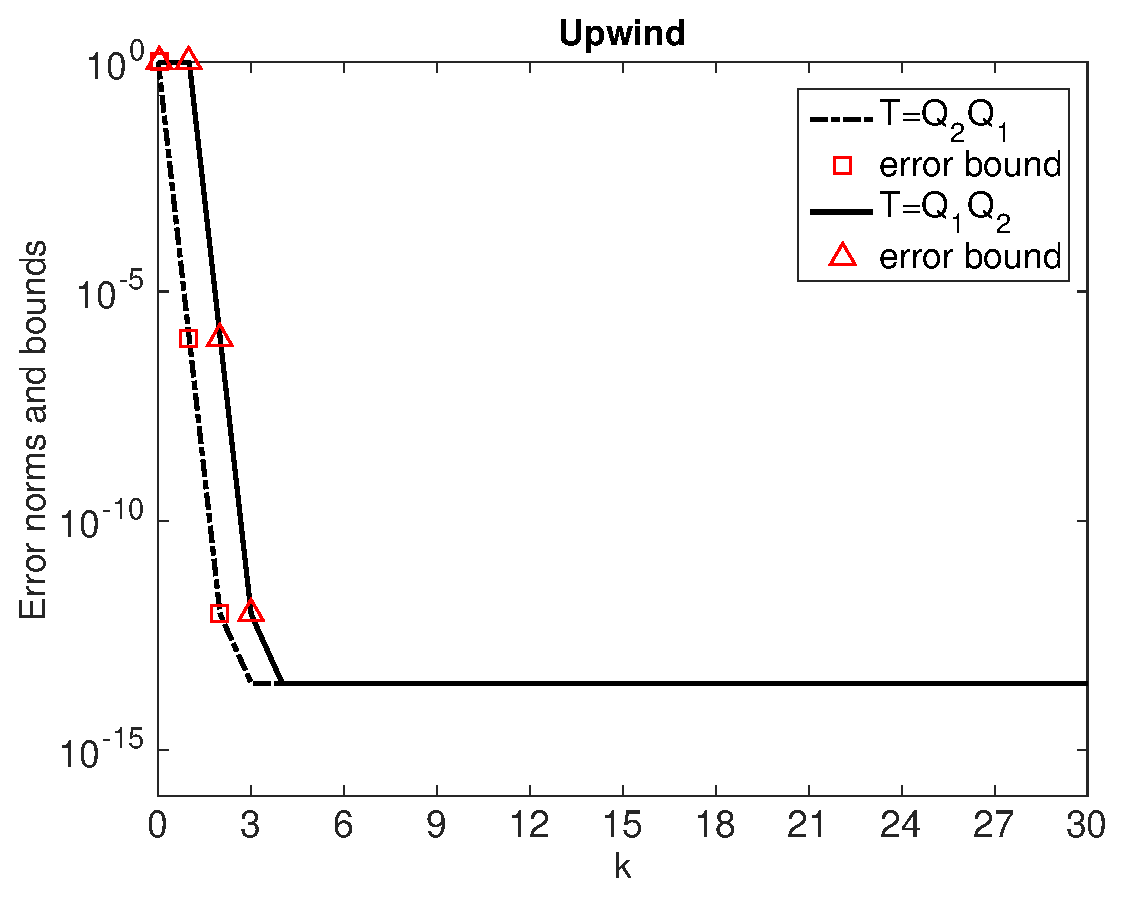
\includegraphics[width=0.95\linewidth]{figures/mSm_upwind_eps_1e-08_N_198}
\end{minipage}
%
\begin{minipage}[t]{0.49\linewidth}
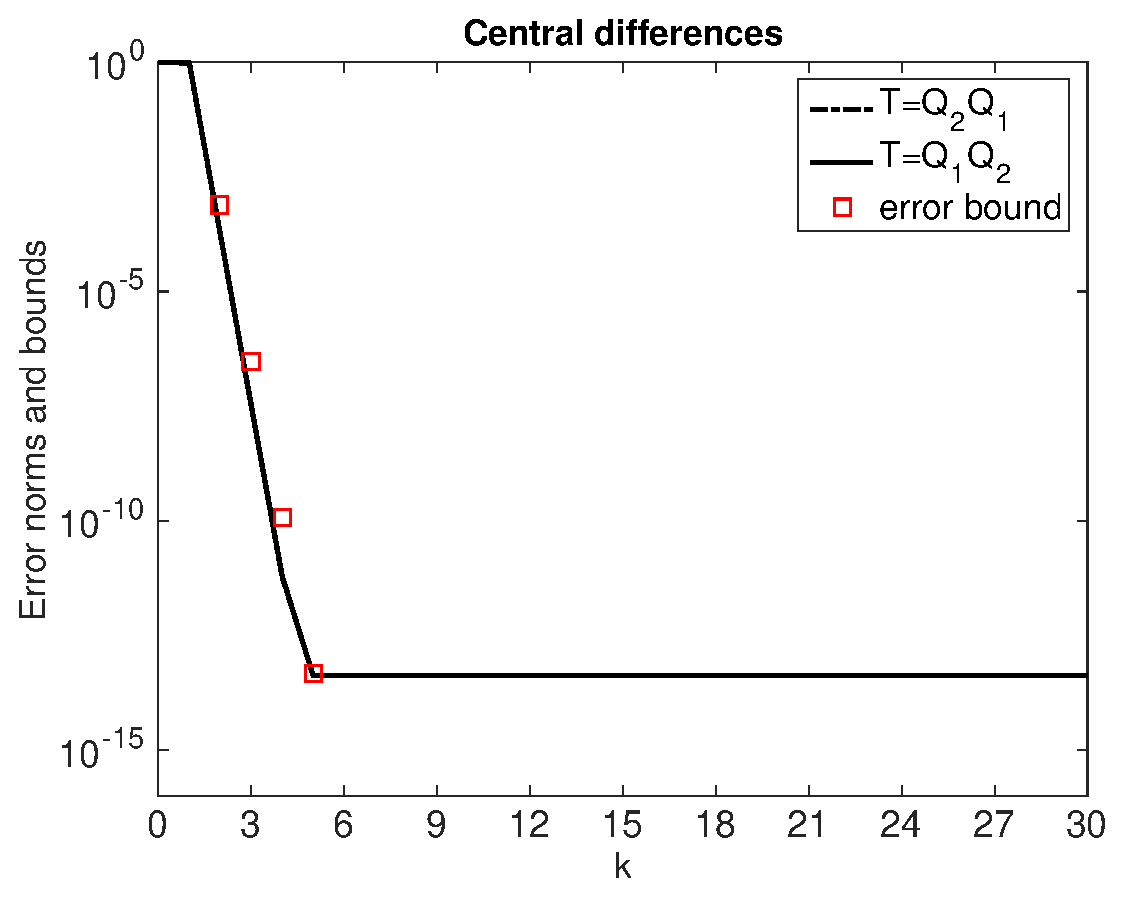
\includegraphics[width=0.95\linewidth]{figures/mSm_central_eps_1e-08_N_198}
\end{minipage}
\caption{Convergence of multiplicative Schwarz and error bounds for
$\epsilon=10^{-8}$, $N=198$, and both discretization schemes.}
%\cblue{Here $|\rho|=9.4\times 10^{-7}<\epsilon(\epsilon+\omega_x H)^{-1}= 9.9 \times 10^{-7}$ for the upwind scheme,
%and $|\rho|=1.8 \times 10^{-4}<2m\epsilon(\epsilon+\omega_x H/2)^{-1}= 3.9 \times 10^{-4}$ for the central differences.}
\label{fig:1D:MSM.N198.eps8}
\end{figure}

\begin{figure}[tbhp]
\begin{minipage}[t]{0.49\linewidth}
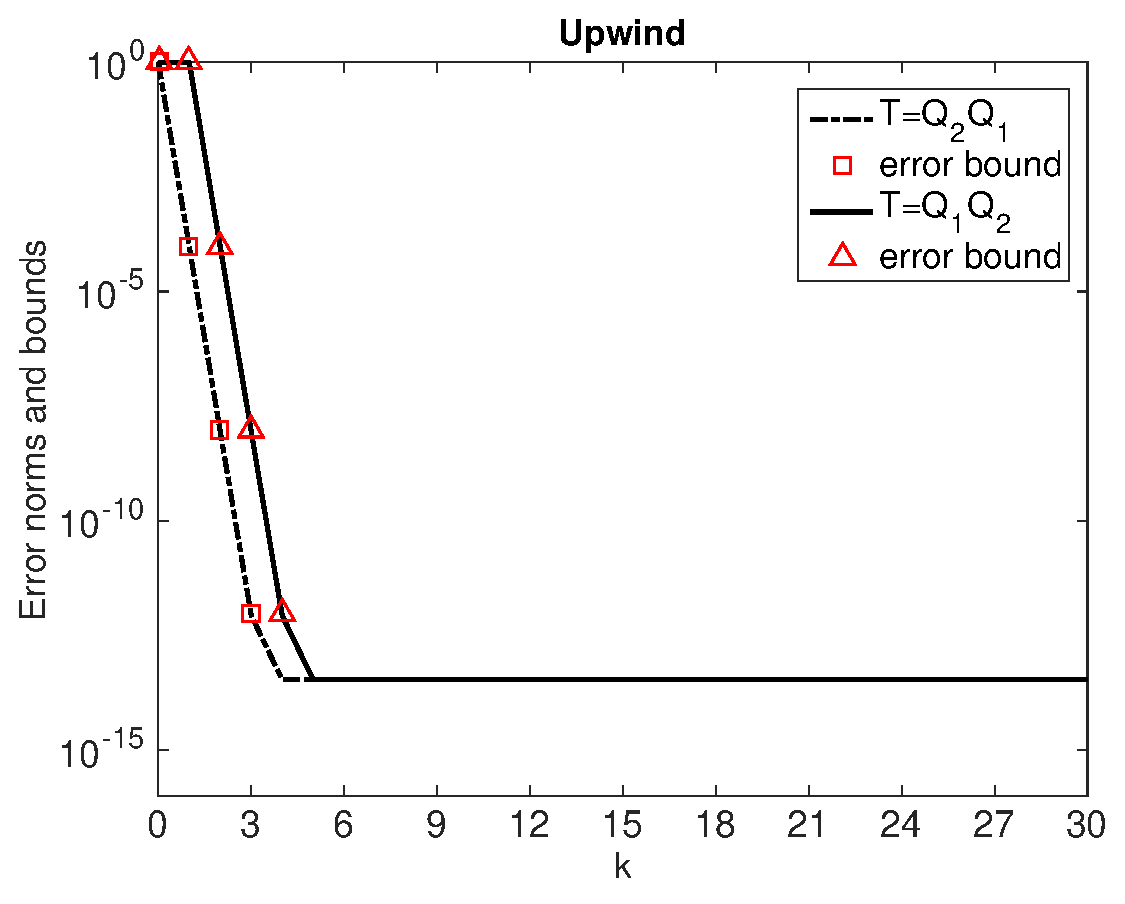
\includegraphics[width=0.95\linewidth]{figures/mSm_upwind_eps_1e-06_N_198}
\end{minipage}
%
\begin{minipage}[t]{0.49\linewidth}
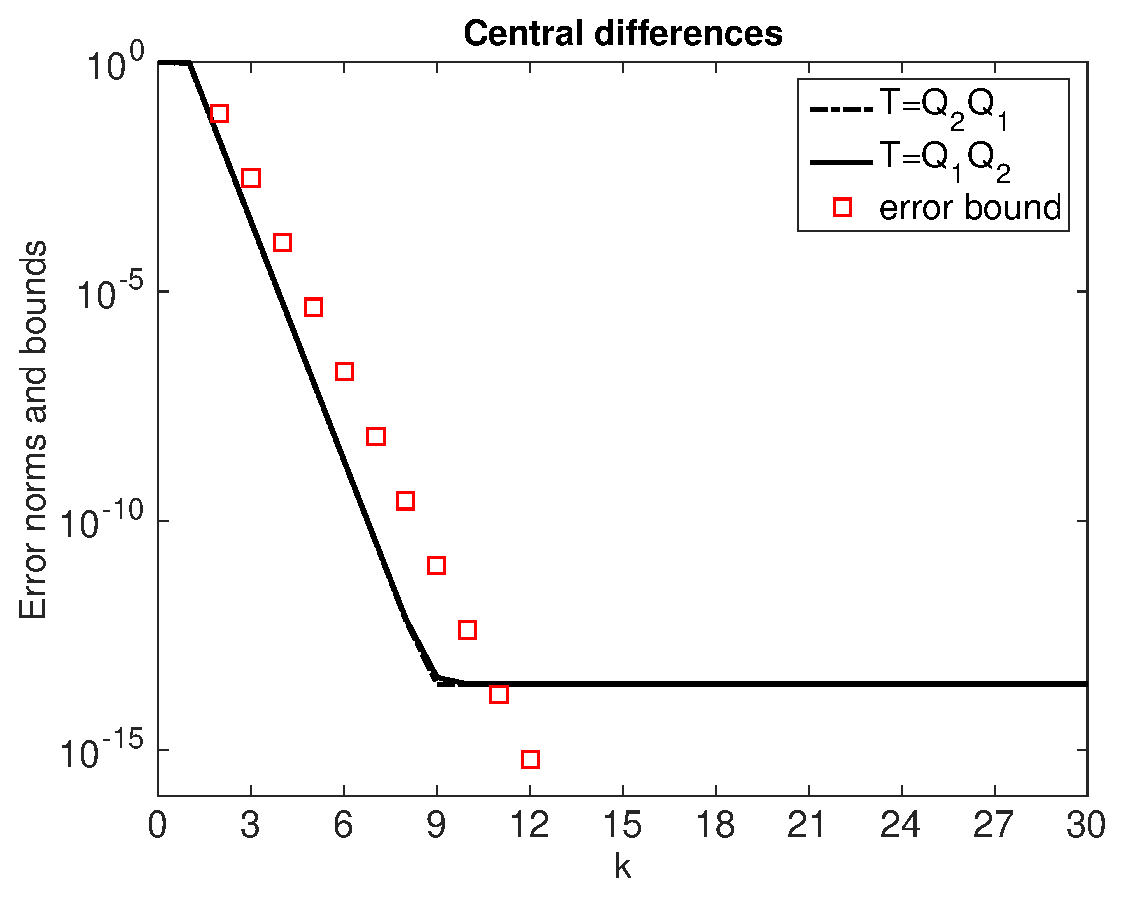
\includegraphics[width=0.95\linewidth]{figures/mSm_central_eps_1e-06_N_198}
\end{minipage}
\caption{Convergence of multiplicative Schwarz and error bounds for
$\epsilon=10^{-6}$, $N=198$, and both discretization schemes.}
%\cblue{Here $|\rho|=9.4\times 10^{-5}<\epsilon(\epsilon+\omega_x H)^{-1}= 9.9 \times 10^{-5}$ for the upwind scheme,
%and $|\rho|=1.8 \times 10^{-2}<2m\epsilon(\epsilon+\omega_x H/2)^{-1}= 3.9 \times 10^{-2}$ for the central differences.}
\label{fig:1D:MSM.N198.eps6}
\end{figure}

\begin{figure}[tbhp]
\begin{minipage}[t]{0.49\linewidth}
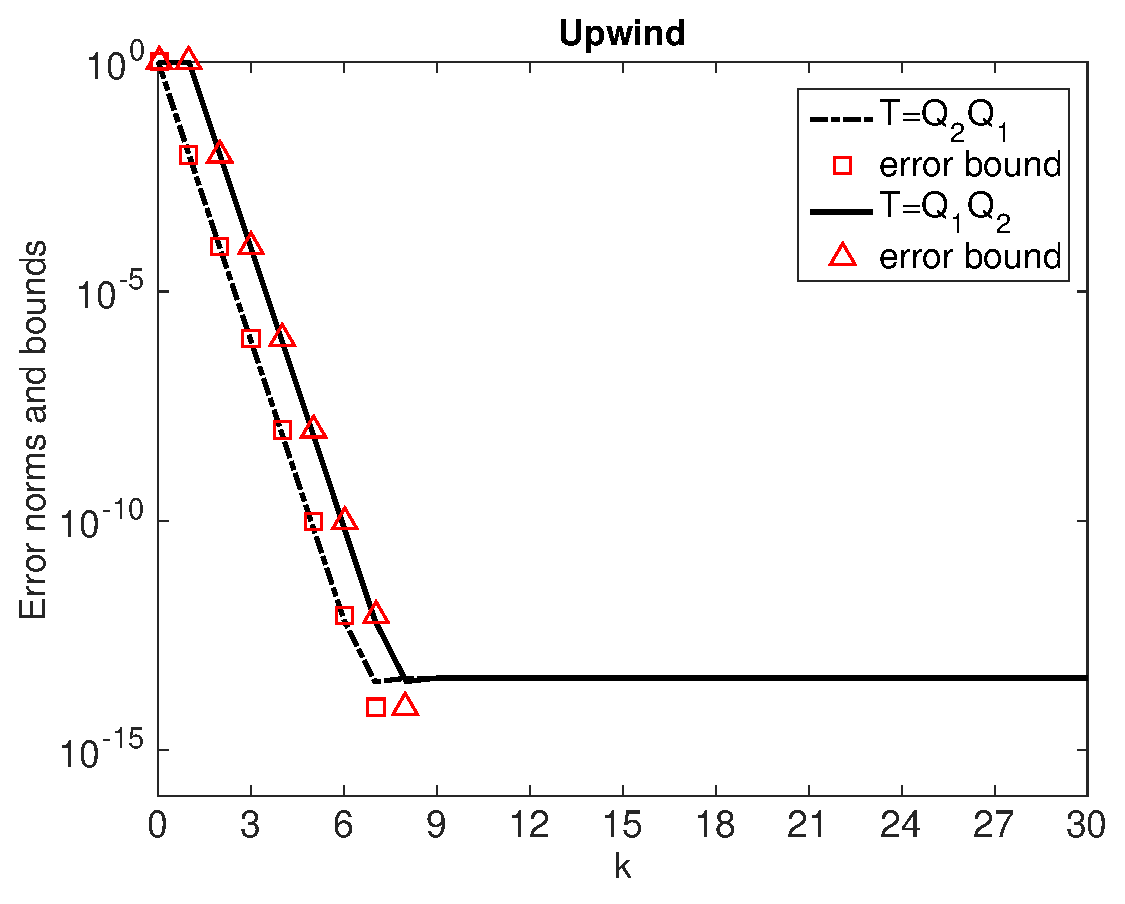
\includegraphics[width=0.95\linewidth]{figures/mSm_upwind_eps_1e-04_N_198}
\end{minipage}
%
\begin{minipage}[t]{0.49\linewidth}
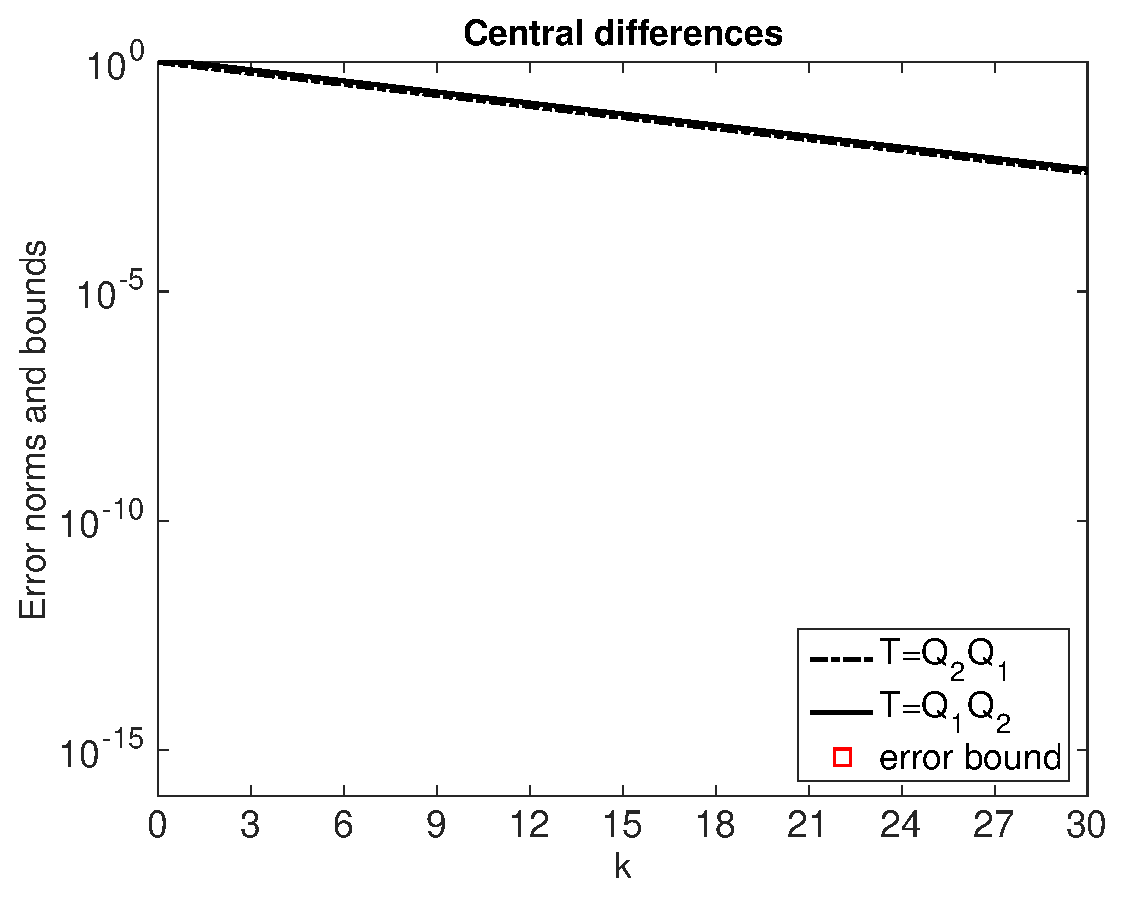
\includegraphics[width=0.95\linewidth]{figures/mSm_central_eps_1e-04_N_198}
\end{minipage}
\caption{Convergence of multiplicative Schwarz and error bounds for
$\epsilon=10^{-4}$, $N=198$, and both discretization schemes.}
%\cblue{Here $|\rho|=9.3\times 10^{-3}<\epsilon(\epsilon+\omega_x H)^{-1}= 9.8 \times 10^{-3}$ for the upwind scheme,
%and $|\rho|=8.3 \times 10^{-1}<2m\epsilon(\epsilon+\omega_x H/2)^{-1}= 3.8$ for the central differences.}
\label{fig:1D:MSM.N198.eps4}
\end{figure}

All numerical results presented in this chapter were performed on a 13-inch
Apple MacBook computer model Mid 2010 with a 2,4 GHz Intel Core 2 Duo
processor. For our experiments we computed $\u=\A^{-1}\f$ using the backslash
operator in \texttt{MATLAB} version R2015b. (Applying iterative refinement in
order to improve the numerical solution obtained in this way yields virtually
the same results, so we do not consider iterative refinement here.) Using the
solution obtained by \texttt{MATLAB}'s backslash, we computed the error norms
of the multiplicative Schwarz method by
$\|\e^{(k)}\|_\infty=\|\u^{(k+1)}-\u\|_\infty$ with $\u^{(k+1)}$
as in \eqref{eq:back:schwarz} and $\u^{(0)}=0$ (rather than using the update
formula $\e^{(k)}=\T_{ij}\e^{(k-1)}$). Consequently, the computed error norms
stagnate on the level of the maximal attainable accuracy of the method.
On the other hand, an error bound of the form $|\rho|^k$ for some
$|\rho|<1$ becomes arbitrarily small for $k\rightarrow\infty$.


\begin{figure}[tbhp]
\begin{minipage}[t]{0.49\linewidth}
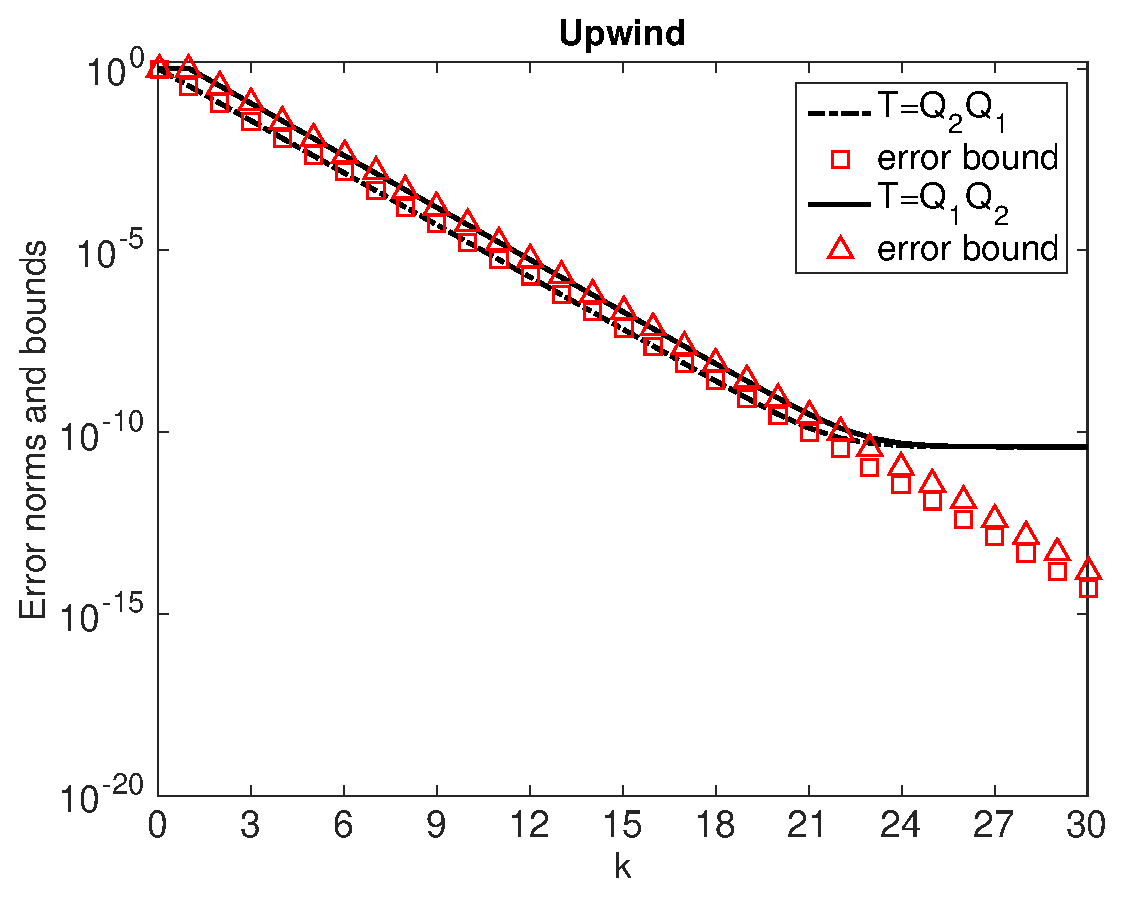
\includegraphics[width=0.95\linewidth]{figures/mSm_upwind_eps_1e-04_N_10002}
\end{minipage}
%
\begin{minipage}[t]{0.49\linewidth}
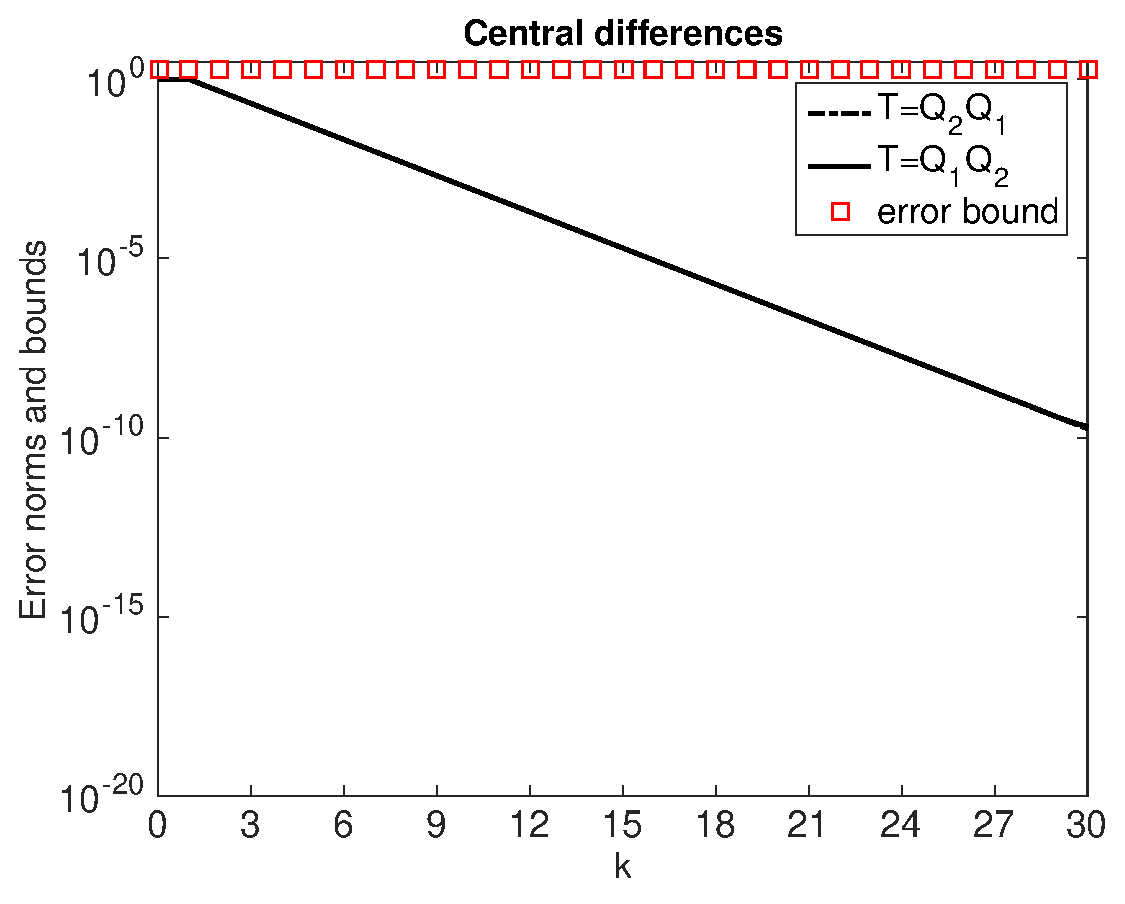
\includegraphics[width=0.95\linewidth]{figures/mSm_central_eps_1e-08_N_10002}
\end{minipage}
\caption{Convergence of multiplicative Schwarz and error bounds for
$\epsilon=10^{-8}$, $N=10002$ and both discretization schemes.}
%\cblue{Here $|\rho|=9.3\times 10^{-3}<\epsilon(\epsilon+\omega_x H)^{-1}= 9.8 \times 10^{-3}$ for the upwind scheme,
%and $|\rho|=8.3 \times 10^{-1}<2m\epsilon(\epsilon+\omega_x H/2)^{-1}= 3.8$ for the central differences.}
\label{fig:1D:MSM.N10002.eps8}
\end{figure}

\begin{figure}[tbhp]
\begin{minipage}[t]{0.49\linewidth}
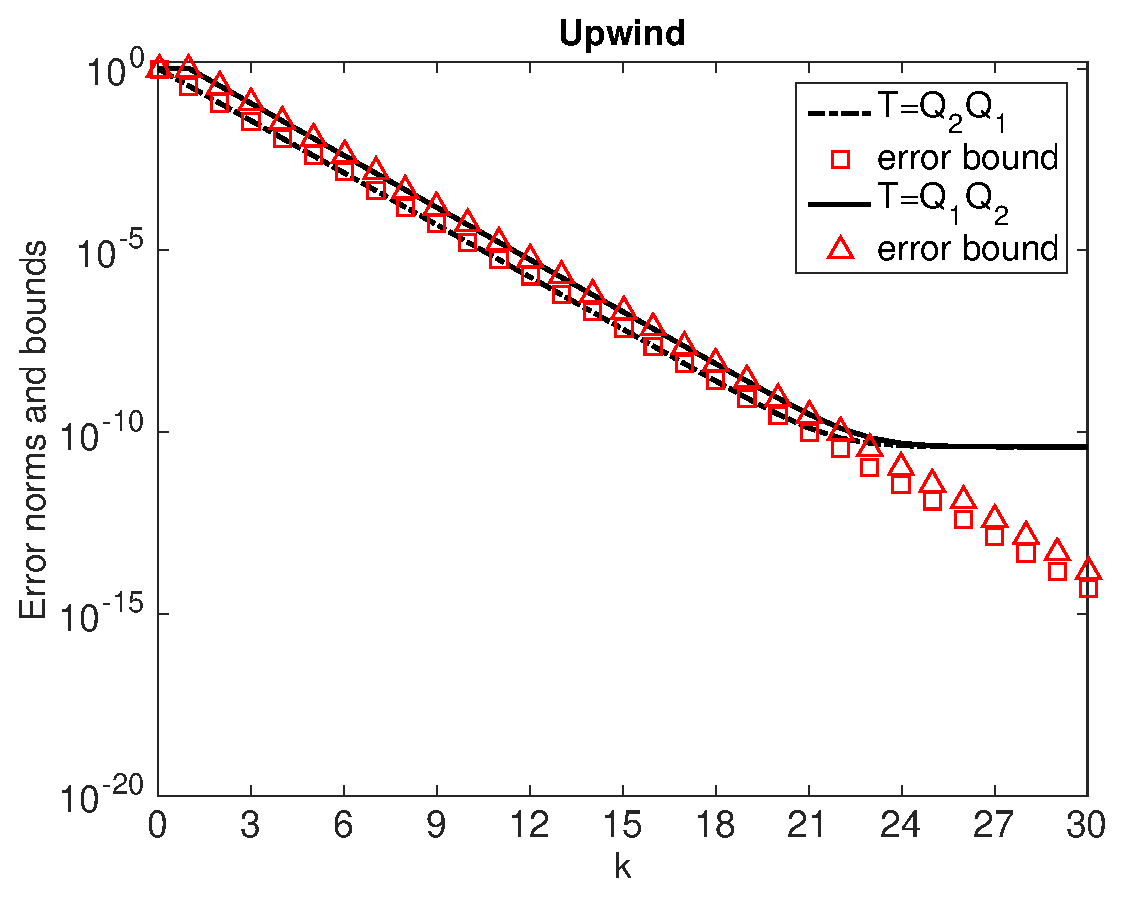
\includegraphics[width=0.95\linewidth]{figures/mSm_upwind_eps_1e-04_N_10002}
\end{minipage}
%
\begin{minipage}[t]{0.49\linewidth}
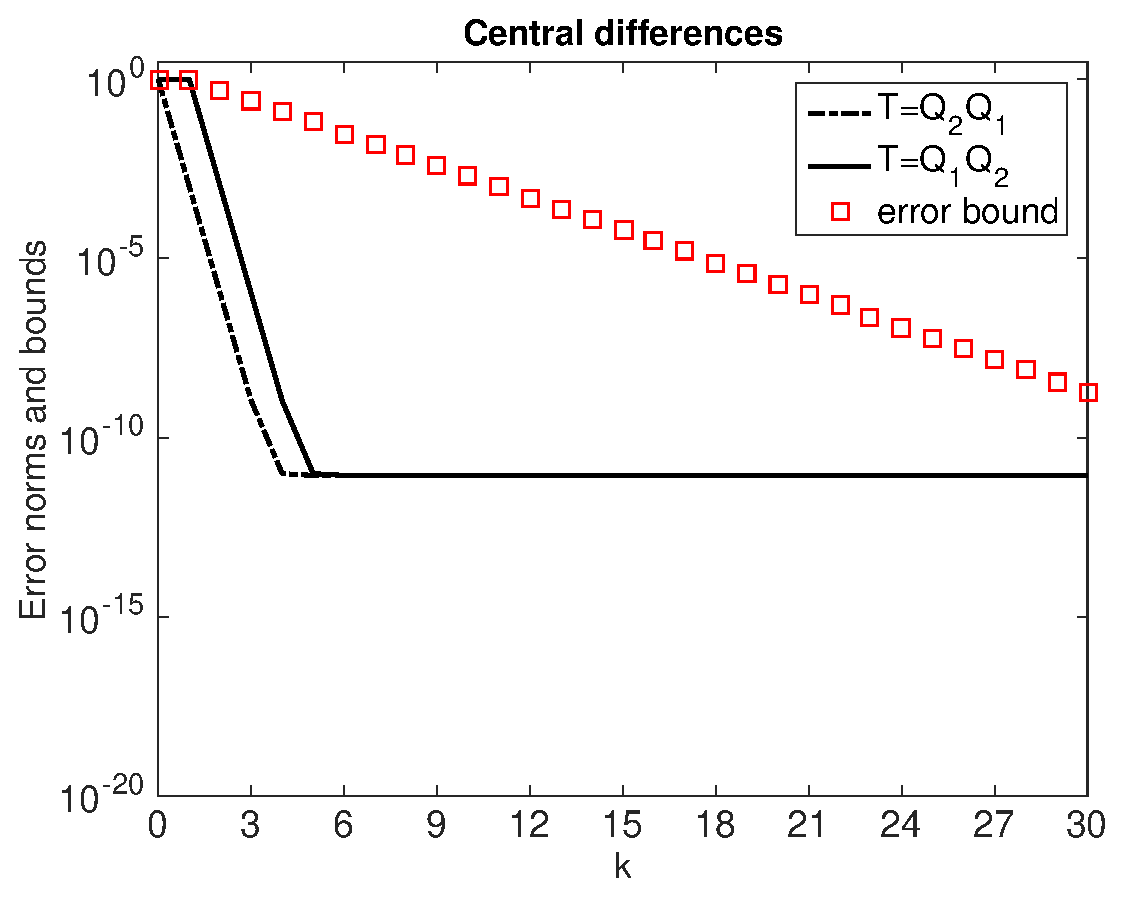
\includegraphics[width=0.95\linewidth]{figures/mSm_central_eps_1e-04_N_10002}
\end{minipage}
\caption{Convergence of multiplicative Schwarz and error bounds for
$\epsilon=10^{-4}$, $N=10002$ and both discretization schemes.}
%\cblue{Here $|\rho|=9.3\times 10^{-3}<\epsilon(\epsilon+\omega_x H)^{-1}= 9.8 \times 10^{-3}$ for the upwind scheme,
%and $|\rho|=8.3 \times 10^{-1}<2m\epsilon(\epsilon+\omega_x H/2)^{-1}= 3.8$ for the central differences.}
\label{fig:1D:MSM.N10002.eps4}
\end{figure}

We start with the upwind discretization. The left parts of
Figures~\ref{fig:1D:MSM.N198.eps8}--\ref{fig:1D:MSM.N10002.eps4}
show the error norms
%
$$\frac{\|\e^{(k)}\|_\infty}{\|\e^{(0)}\|_\infty},\quad  k=0,1,2\dots,$$
%
for the iteration matrices $\T_{12}$ (solid) and $\T_{21}$
(dashed) as well as the corresponding upper bounds from
Theorem~\ref{thm:1D:upwind_conv},
for increasing values of $\epsilon$. We observe that the bounds are
quite close to the actual errors. Moreover, in each case the error norm for
the multiplicative Schwarz method with the iteration matrix $\T_{21}$
almost stagnates in the first step, as predicted by the bound in
Theorem~\ref{thm:1D:upwind_conv}.

On the right parts of Figures~\ref{fig:1D:MSM.N198.eps8}--\ref{fig:1D:MSM.N10002.eps4} we show the
error norms of the multiplicative Schwarz method and the corresponding
convergence bounds from Theorem~\ref{thm:1D:central_conv} for the central
difference scheme.
For our choice of parameters we have $\omega_x H > 2\epsilon$. Note that the
error norms are virtually the same for both iteration matrices. However,
the bounds are not as tight as for the upwind scheme. For fixed $N$ the bounds
become weaker with increasing $\epsilon$, i.e., decreasing convection-
dominance. For our chosen parameters and $\epsilon=10^{-4}$,
giving $\epsilon N^2=\mathscr{O}(1)$, the convergence of the multiplicative
Schwarz method becomes very slow, and the bound~(\ref{eq:1D:bound2}) fails to
predict convergence at all.

We also run the experiments for larger values of $N$. The values of $|\rho|$
and the corresponding bounds from Theorems~\ref{thm:1D:upwind_conv} and
\ref{thm:1D:central_conv} are shown in Table~\ref{tab:1D:rho} for different
values of $N$. We observe that for all cases the bounds on $|\rho|$ for the
upwind scheme are  tighter than for the central difference scheme.
%
\begin{table}[tbhp]
\centering
%\begin{tabular}{rc|c||c|c}
\begin{tabular}{r|c c |c c}
\cline{1-5}
%   & \multicolumn{2}{ c | }{upwind} & \multicolumn{2}{ c }{central differences}\\ \hline
% \multicolumn{1}{ c|   }{$\epsilon$}&$|\rho|$~\eqref{eq:1D:rho} & bound~\eqref{eq:1D:bound_upw} & $|\rho|$~\eqref{eq:1D:rho} & bound~\eqref{eq:1D:bound2}\\
%\hline
\multicolumn{5}{c}{$N=66$}\\\hline
%\multicolumn{1}{ c|  }{$10^{-9}$} & $2.9 \times 10^{-8}$ & $3.3 \times 10^{-8}$ & $1.8 \times 10^{-6}$ & $4.2 \times 10^{-6}$\\
\multicolumn{1}{ c|  }{$10^{-8}$} & $2.9 \times 10^{-7}$ & $3.3 \times 10^{-7}$ & $1.8 \times 10^{-5}$ & $4.2 \times 10^{-5}$\\
\multicolumn{1}{ c|  }{$10^{-6}$} & $2.9 \times 10^{-5}$ & $3.3 \times 10^{-5}$ & $1.8\times 10^{-3}$ & $4.2\times 10^{-3}$\\
\multicolumn{1}{ c|  }{$10^{-4}$} & $2.9 \times 10^{-3}$ & $3.3 \times 10^{-3}$ & $1.8\times 10^{-1}$ & $4.2\times 10^{-1}$\\
\multicolumn{1}{ c|  }{$10^{-2}$} & $2.3 \times 10^{-1}$ & $2.6 \times 10^{-1}$ & $1.3\times 10^{-1}$ & $2.7\times 10^{+1}$\\ \hline
\multicolumn{5}{c}{$N=130$}\\\hline
%\multicolumn{1}{ c|  }{$10^{-9}$} & $6.0 \times 10^{-8}$ & $6.5 \times 10^{-8}$ & $7.7 \times 10^{-6}$ & $1.7 \times 10^{-5}$\\
\multicolumn{1}{ c|  }{$10^{-8}$} & $6.0 \times 10^{-7}$ & $6.5 \times 10^{-7}$ & $7.7 \times 10^{-5}$ & $1.7 \times 10^{-4}$\\
\multicolumn{1}{ c|  }{$10^{-6}$} & $6.0 \times 10^{-5}$ & $6.5 \times 10^{-5}$ & $7.7\times 10^{-3}$ & $1.7\times 10^{-2}$\\
\multicolumn{1}{ c|  }{$10^{-4}$} & $6.0 \times 10^{-3}$ & $6.5 \times 10^{-3}$ & $5.9\times 10^{-1}$ & $1.6\times 10^{~0}$\\
\multicolumn{1}{ c|  }{$10^{-2}$} & $3.8 \times 10^{-1}$ & $4.2 \times 10^{-1}$ & $1.6\times 10^{-1}$ & $5.7\times 10^{-1}$\\ \hline
\multicolumn{5}{c}{$N=258$}\\\hline
%\multicolumn{1}{ c|  }{$10^{-9}$} & $1.2 \times 10^{-7}$ & $1.3 \times 10^{-7}$ & $3.2 \times 10^{-5}$ & $6.6 \times 10^{-5}$\\
\multicolumn{1}{ c|  }{$10^{-8}$} & $1.2 \times 10^{-6}$ & $1.3 \times 10^{-6}$ & $3.2 \times 10^{-4}$ & $6.6 \times 10^{-4}$\\
\multicolumn{1}{ c|  }{$10^{-6}$} & $1.2 \times 10^{-4}$ & $1.3 \times 10^{-4}$ & $3.2\times 10^{-2}$ & $6.6\times 10^{-2}$\\
\multicolumn{1}{ c|  }{$10^{-4}$} & $1.2 \times 10^{-2}$ & $1.3 \times 10^{-2}$ & $8.7\times 10^{-1}$ & $6.4\times 10^{~0}$\\
\multicolumn{1}{ c|  }{$10^{-2}$} & $5.5 \times 10^{-1}$ & $5.9 \times 10^{-1}$ & $4.5\times 10^{-1}$ & $7.2\times 10^{-1}$\\ \hline
\multicolumn{5}{c}{$N=514$}\\\hline
%\multicolumn{1}{ c|  }{$10^{-9}$} & $2.5 \times 10^{-7}$ & $2.6 \times 10^{-7}$ & $1.3 \times 10^{-4}$ & $2.6 \times 10^{-4}$\\
\multicolumn{1}{ c|  }{$10^{-8}$} & $2.5 \times 10^{-6}$ & $2.6 \times 10^{-6}$ & $1.3 \times 10^{-3}$ & $2.6 \times 10^{-3}$\\
\multicolumn{1}{ c|  }{$10^{-6}$} & $2.5 \times 10^{-4}$ & $2.6 \times 10^{-4}$ & $1.3\times 10^{-1}$ & $2.6\times 10^{-1}$\\
\multicolumn{1}{ c|  }{$10^{-4}$} & $2.4 \times 10^{-2}$ & $2.5 \times 10^{-2}$ & $8.6\times 10^{-1}$ & $2.5\times 10^{+1}$\\
\multicolumn{1}{ c|  }{$10^{-2}$} & $7.2 \times 10^{-1}$ & $7.5 \times 10^{-1}$ & $6.8\times 10^{-1}$ & $8.4\times 10^{-1}$\\ \hline
\multicolumn{5}{c}{$N=1026$}\\\hline
%\multicolumn{1}{ c|  }{$10^{-9}$} & $5.1 \times 10^{-7}$ & $5.1 \times 10^{-7}$ & $5.2 \times 10^{-4}$ & $1.1 \times 10^{-3}$\\
\multicolumn{1}{ c|  }{$10^{-8}$} & $5.1 \times 10^{-6}$ & $5.1 \times 10^{-6}$ & $5.2 \times 10^{-3}$ & $1.1 \times 10^{-2}$\\
\multicolumn{1}{ c|  }{$10^{-6}$} & $5.1 \times 10^{-4}$ & $5.1 \times 10^{-4}$ & $4.7\times 10^{-1}$ & $1.0\times 10^{~0}$\\
\multicolumn{1}{ c|  }{$10^{-4}$} & $4.8 \times 10^{-2}$ & $4.9 \times 10^{-2}$ & $7.9\times 10^{-1}$ & $9.5\times 10^{+1}$\\
\multicolumn{1}{ c|  }{$10^{-2}$} & $8.4 \times 10^{-1}$ & $8.6 \times 10^{-1}$ & $8.2\times 10^{-1}$ & $9.1   \times 10^{-1}$\\ \hline
\multicolumn{5}{c}{$N=2050$}\\\hline
%\multicolumn{1}{ c|  }{$10^{-9}$} & $1.0 \times 10^{-6}$ & $1.0 \times 10^{-6}$ & $2.1 \times 10^{-3}$ & $4.2 \times 10^{-3}$\\
\multicolumn{1}{ c|  }{$10^{-8}$} & $1.0 \times 10^{-5}$ & $1.0 \times 10^{-5}$ & $2.1 \times 10^{-2}$ & $4.2 \times 10^{-2}$\\
\multicolumn{1}{ c|  }{$10^{-6}$} & $1.0 \times 10^{-3}$ & $1.0 \times 10^{-3}$ & $9.5\times 10^{-1}$ & $4.2\times 10^{~0}$\\
\multicolumn{1}{ c|  }{$10^{-4}$} & $9.2 \times 10^{-2}$ & $9.3 \times 10^{-2}$ & $6.5\times 10^{-1}$ & $3.5\times 10^{+2}$\\
\multicolumn{1}{ c|  }{$10^{-2}$} & $9.1 \times 10^{-1}$ & $9.2 \times 10^{-1}$ & $9.1\times 10^{-1}$ & $9.5   \times 10^{-1}$\\ \hline
\multicolumn{5}{c}{$N=4098$}\\\hline
%\multicolumn{1}{ c|  }{$10^{-9}$} & $2.0 \times 10^{-6}$ & $2.0 \times 10^{-6}$ & $8.4 \times 10^{-3}$ & $1.7 \times 10^{-2}$\\
\multicolumn{1}{ c|  }{$10^{-8}$} & $2.0 \times 10^{-5}$ & $2.0 \times 10^{-5}$ & $8.3 \times 10^{-2}$ & $1.7 \times 10^{-1}$\\
\multicolumn{1}{ c|  }{$10^{-6}$} & $2.0 \times 10^{-3}$ & $2.0 \times 10^{-3}$ & $9.8\times 10^{-1}$ & $1.7\times 10^{+1}$\\
\multicolumn{1}{ c|  }{$10^{-4}$} & $1.7 \times 10^{-1}$ & $1.7 \times 10^{-1}$ & $4.1\times 10^{-1}$ & $1.2\times 10^{+3}$\\
\multicolumn{1}{ c|  }{$10^{-2}$} & $9.5 \times 10^{-1}$ & $9.6 \times 10^{-1}$ & $9.5\times 10^{-1}$ & $9.8   \times 10^{-1}$\\ \hline
\multicolumn{5}{c}{$N=8194$}\\\hline
\multicolumn{1}{ c|  }{$10^{-8}$} & $4.1 \times 10^{-5}$ & $4.1 \times 10^{-5}$ & $3.2 \times 10^{-1}$ & $6.7 \times 10^{-1}$\\
\multicolumn{1}{ c|  }{$10^{-6}$} & $4.1 \times 10^{-3}$ & $4.1 \times 10^{-3}$ & $9.8 \times 10^{-1}$ & $6.7 \times 10^{+1}$\\
\multicolumn{1}{ c|  }{$10^{-4}$} & $2.9 \times 10^{-1}$ & $2.9 \times 10^{-1}$ & $9.8 \times 10^{-2}$ & $3.7 \times 10^{+3}$\\
\multicolumn{1}{ c|  }{$10^{-2}$} & $9.8 \times 10^{-1}$ & $9.8 \times 10^{-1}$ & $9.8 \times 10^{-1}$ & $9.9 \times 10^{-1}$\\
% & \multicolumn{2}{ c | }{upwind} & \multicolumn{2}{ c }{central differences}\\
%\hline
\multicolumn{1}{ c|   }{$\epsilon$}&$|\rho|$~\eqref{eq:1D:rho} & bound~\eqref{eq:1D:bound_upw} & $|\rho|$~\eqref{eq:1D:rho} & bound~\eqref{eq:1D:bound2}\\ \hline
& \multicolumn{2}{ c | }{upwind} & \multicolumn{2}{ c }{central differences}\\
\hline
\end{tabular}
\caption{Values of $|\rho|$ computed using \eqref{eq:1D:rho} and the corresponding bounds (\ref{eq:1D:bound_upw}) and (\ref{eq:1D:bound2}) for different values of $\epsilon$ and $N$.}
\label{tab:1D:rho}
\end{table}

To further illustrate our results, we also present the results for a larger
value of $N$, namely $N=10002$. We consider the special cases
$\epsilon N^2 \approx 1$ (Figure~\ref{fig:1D:MSM.N10002.eps8})
and $\epsilon N \approx 1$ (Figure~\ref{fig:1D:MSM.N10002.eps4})
which are mainly of theoretical interest. While the bound
\eqref{eq:1D:bound_upw} for the upwind scheme is still tight and descriptive,
the bound~\eqref{eq:1D:bound2} for the central difference scheme does not
predict convergence well. Note that the parameters used in
Figure~\ref{fig:1D:MSM.N10002.eps4} yield
$\omega_x H\approx 1.9959\times 10^{-4} < 2\epsilon$, and hence the right part
of Figure~\ref{fig:1D:MSM.N10002.eps4} shows error norms and the convergence
bound corresponding to the case $\omega_x H\leq 2\epsilon$ in
Theorem~\ref{thm:1D:central_conv}.

We continue our numerical experiments by applying GMRES to the linear
algebraic system \emph{preconditioned with multiplicative Schwarz}, i.e., the
linear algebraic system \eqref{eq:1D:precond}, in the case $N=198$. Using the
2-norm, the (preconditioned) relative residual norms are shown in
Figures~\ref{fig:1D:GMRES.N198.eps6.prec}--\ref{fig:1D:GMRES.N198.eps8.prec}
and were computed using \texttt{MATLAB}'s command \texttt{gmres} with a
tolerance of $10^{-14}$, a maximum number of iterations of $N-1$ and initial
approximation $\u^{(0)}=0$. In all cases convergence is achieved in two
iterations, which is explained in the previous section. These figures are the
counterparts to
Figures~\ref{fig:back:GMRES.N198.eps4}--\ref{fig:back:GMRES.N198.eps8},
where GMRES makes little progress until iteration 198.

\begin{figure}[tbhp]
\begin{minipage}[t]{0.48\linewidth}
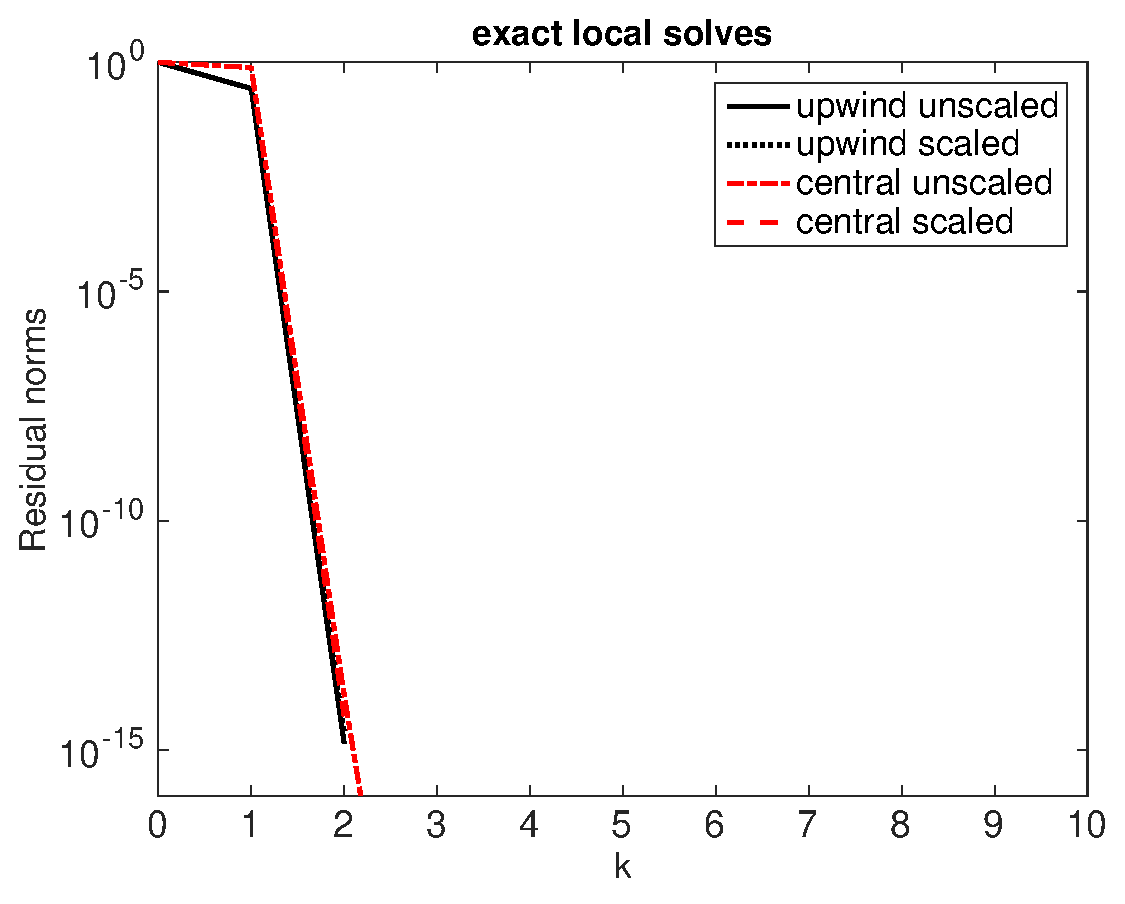
\includegraphics[width=0.98\linewidth]{figures/gmres_eps_1e-02_N_198_prec}
%\label{fig:1D:GMRES.N198.eps4.prec}
% note: if changing to 3 figures again, it needs to be changed in two places
%\caption{Preconditioned GMRES convergence for $\epsilon=10^{-4}$.}
\end{minipage}
%
\begin{minipage}[t]{0.48\linewidth}
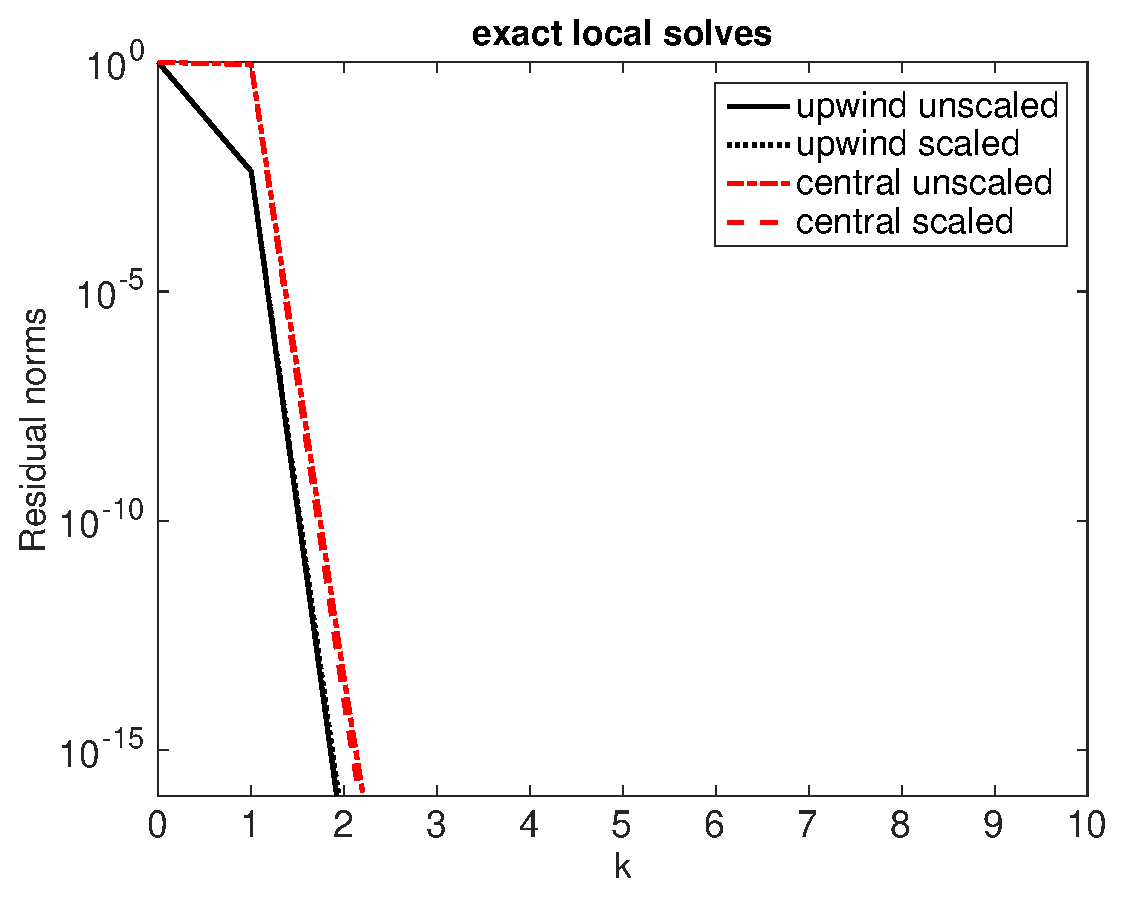
\includegraphics[width=0.98\linewidth]{figures/gmres_eps_1e-04_N_198_prec}
\end{minipage}
\caption{Preconditioned GMRES convergence for $\epsilon=10^{-2}$ [l.] and $\epsilon=10^{-4}$ [r.]}
\label{fig:1D:GMRES.N198.eps6.prec}
\end{figure}
%
\begin{figure}[tbhp]
\begin{minipage}[t]{0.48\linewidth}
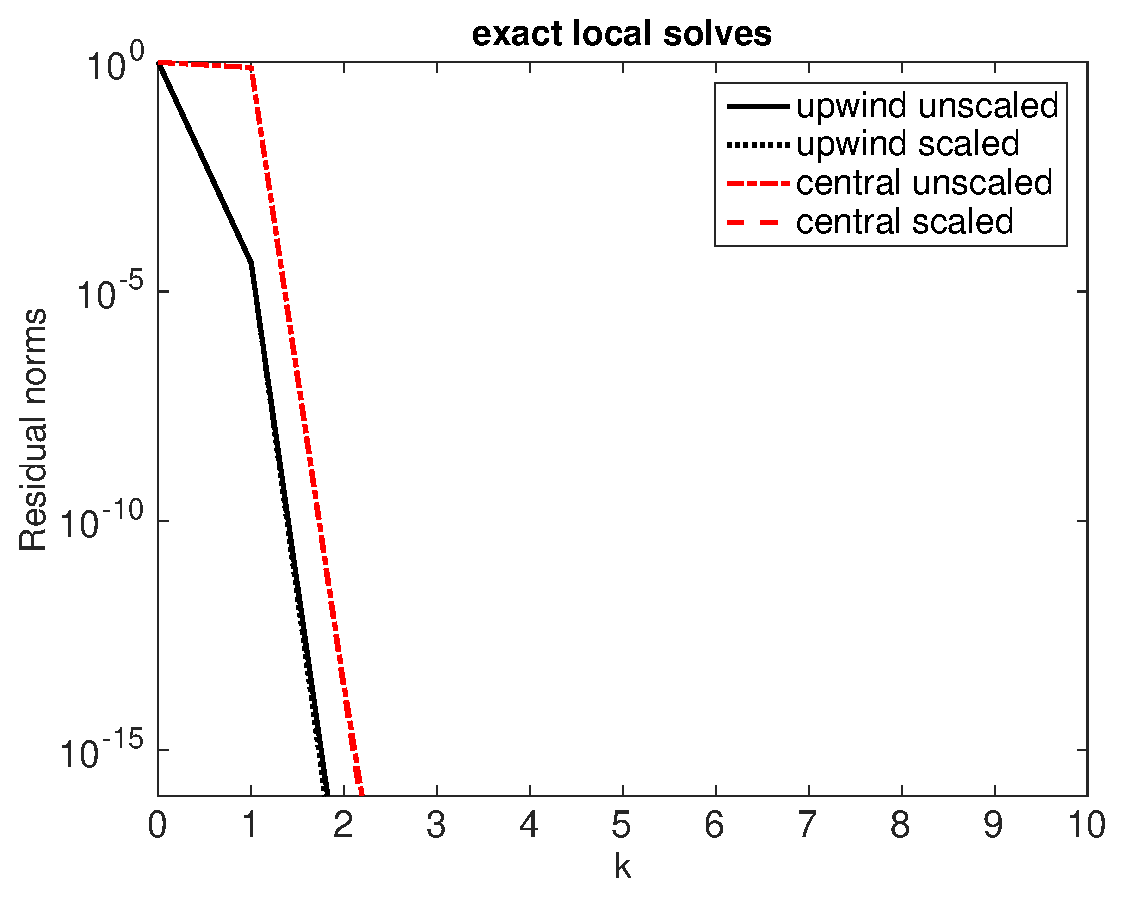
\includegraphics[width=0.98\linewidth]{figures/gmres_eps_1e-06_N_198_prec}
%\label{fig:1D:GMRES.N198.eps4.prec}
% note: if changing to 3 figures again, it needs to be changed in two places
%\caption{Preconditioned GMRES convergence for $\epsilon=10^{-4}$.}
\end{minipage}
%
\begin{minipage}[t]{0.48\linewidth}
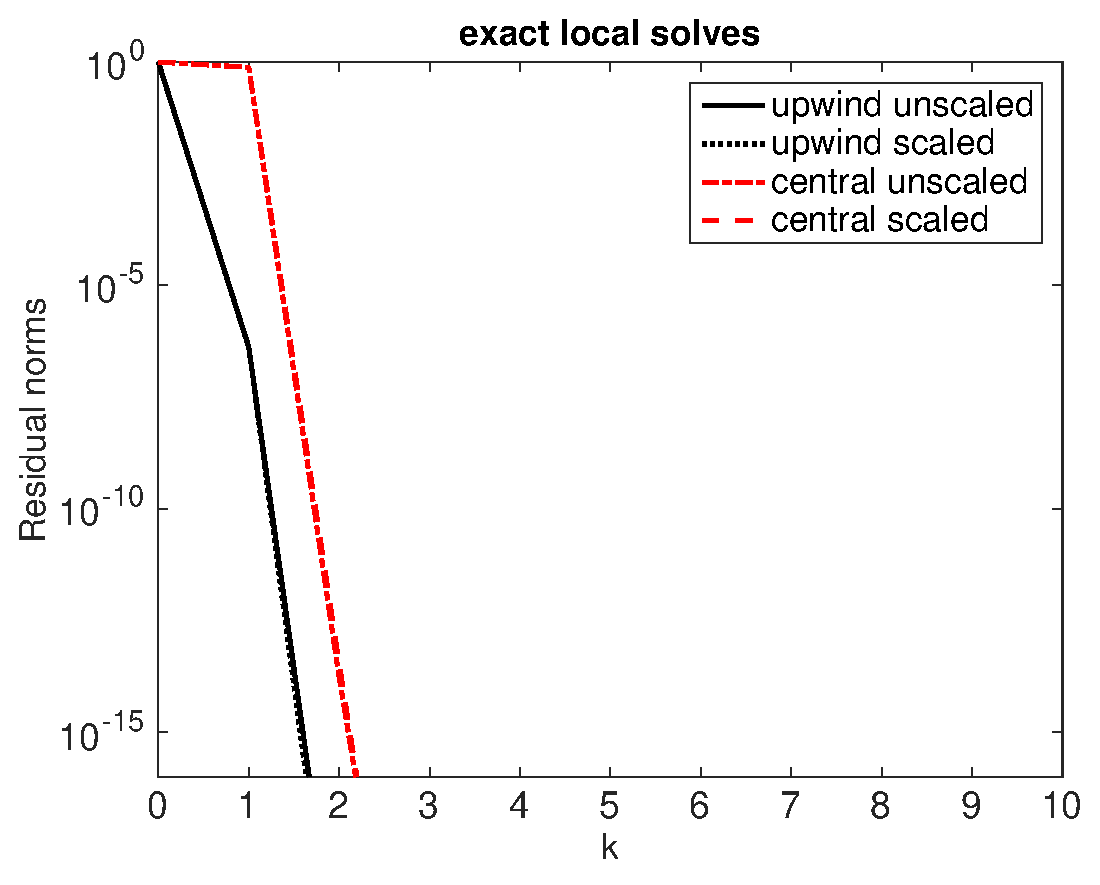
\includegraphics[width=0.98\linewidth]{figures/gmres_eps_1e-08_N_198_prec}
\end{minipage}
\caption{Preconditioned GMRES convergence for $\epsilon=10^{-6}$ [l.] and $\epsilon=10^{-8}$ [r.].}
\label{fig:1D:GMRES.N198.eps8.prec}
\end{figure}
%
% \begin{figure}[h!]
% \hspace{-1cm}
% \centering
% \begin{minipage}[t]{0.78\linewidth}
% \centering
% 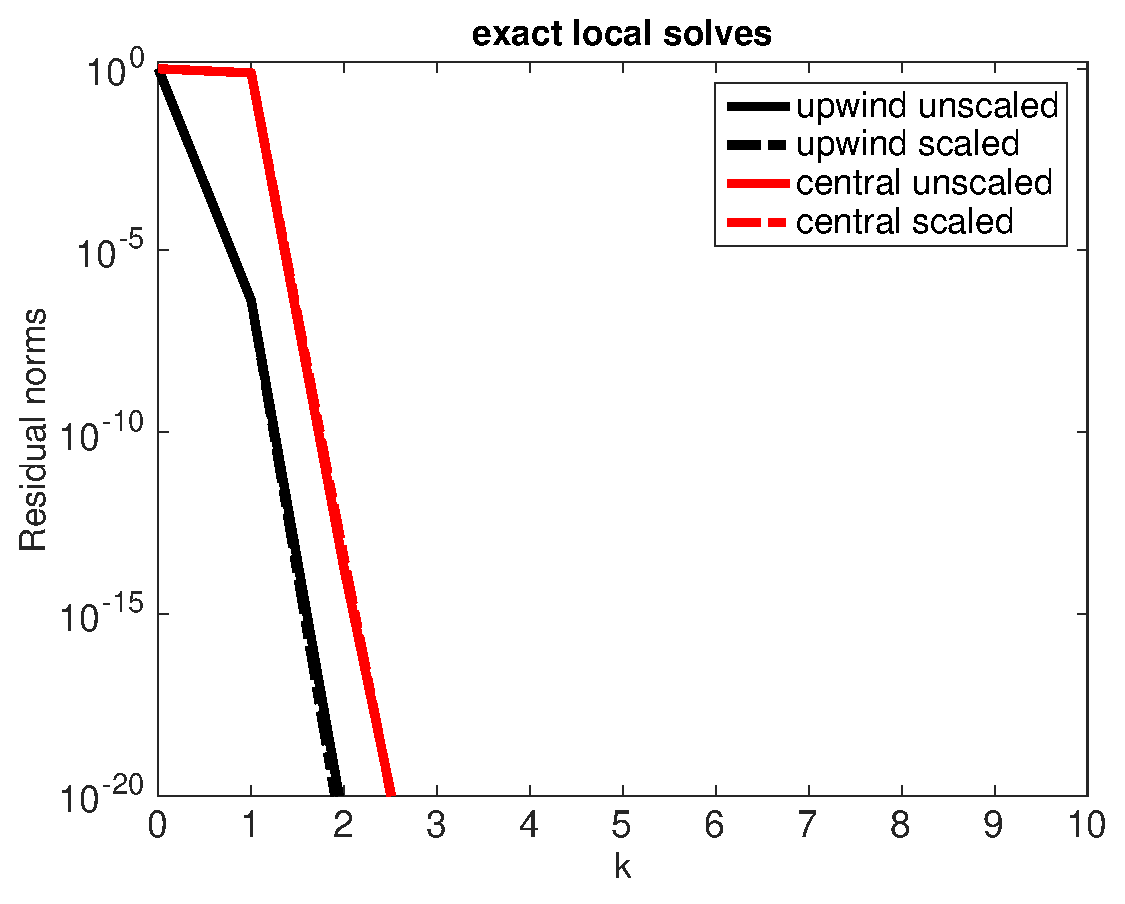
\includegraphics[width=0.6\linewidth]{figures/gmres_8_198_prec}
% \caption{Preconditioned GMRES convergence for $\epsilon~=~10^{-8}$.}
% \label{fig:1D:GMRES.N198.eps8.prec}
% \end{minipage}
% \end{figure}

% \begin{figure}[tbhp]
% \begin{minipage}[t]{0.48\linewidth}
% 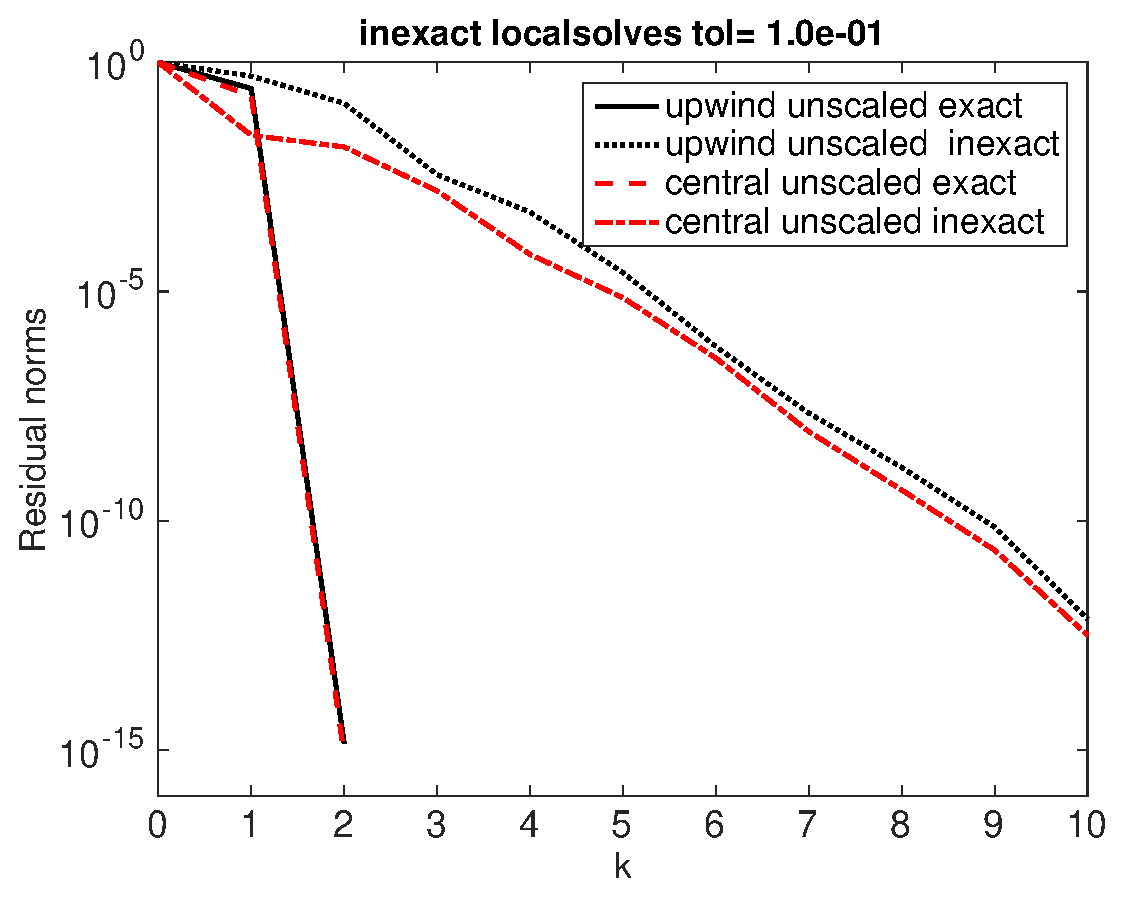
\includegraphics[width=0.98\linewidth]{figures/gmres_8_198_inexact-1e-01}
% %\label{fig:1D:GMRES.N198.eps4.prec}
% % note: if changing to 3 figures again, it needs to be changed in two places
% %\caption{Preconditioned GMRES convergence for $\epsilon=10^{-4}$.}
% \end{minipage}
% %
% \begin{minipage}[t]{0.48\linewidth}
% 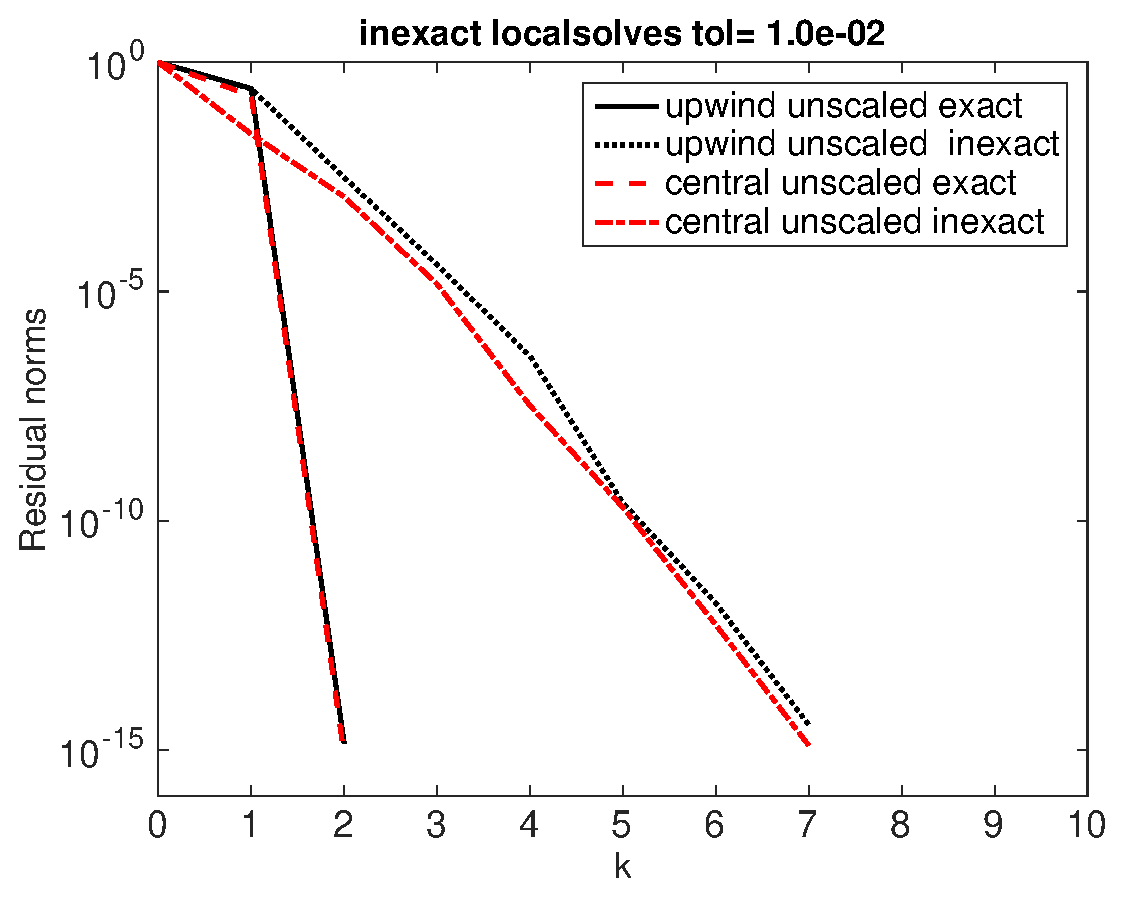
\includegraphics[width=0.98\linewidth]{figures/gmres_8_198_inexact-1e-02}
% \end{minipage}
% \caption{Preconditioned GMRES convergence for $\epsilon~=~10^{-8}$ [l.] with inexact local solve tolerance of $10^{-1}$ and $10^{-2}$ [r.].}
% \label{fig:1D:GMRES.inexact.prec.N198.eps8.tol1_2}
% \end{figure}
% %
% \begin{figure}[tbhp]
% \hspace{-1cm}
% \centering
% \begin{minipage}[t]{0.48\linewidth}
% \centering
% 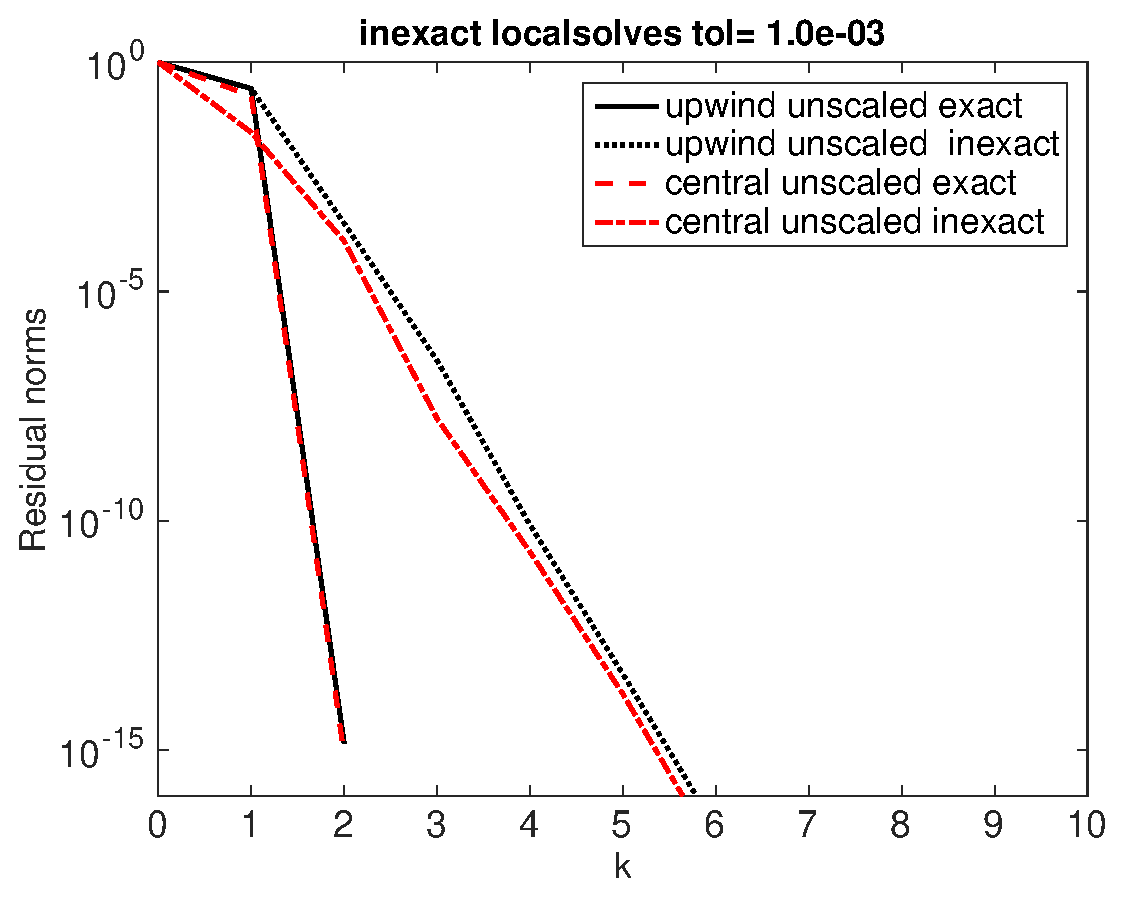
\includegraphics[width=0.98\linewidth]{figures/gmres_8_198_inexact-1e-03}
% \end{minipage}
% %
% \begin{minipage}[t]{0.48\linewidth}
% 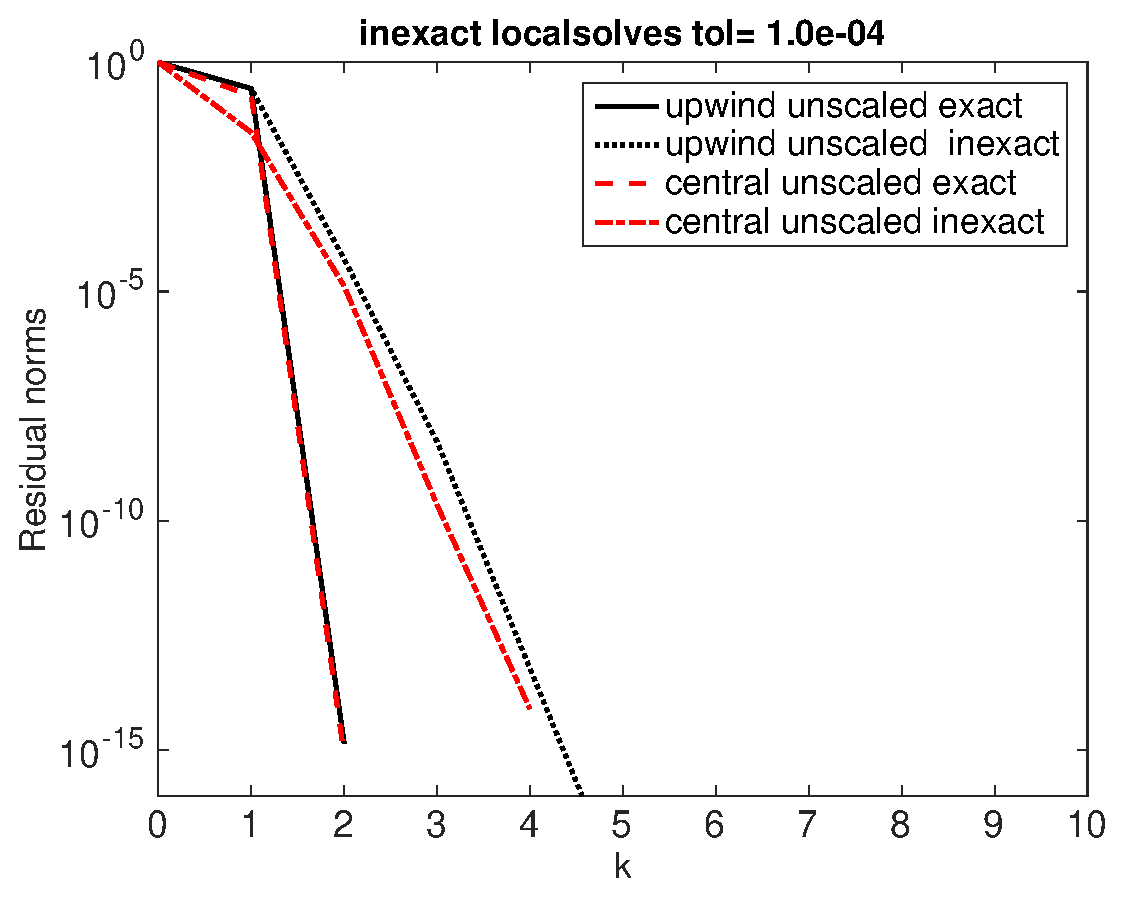
\includegraphics[width=0.98\linewidth]{figures/gmres_8_198_inexact-1e-04}
% \end{minipage}
% \caption{Preconditioned GMRES convergence for $\epsilon~=~10^{-8}$ with inexact local solve tolerance of $10^{-3}$ [l.] and $10^{-4}$ [r.].}
% \label{fig:1D:GMRES.inexact.prec.N198.eps8.tol3_4}
% \end{figure}
%
% We conclude our numerical experiments by presenting results for the
% preconditioned GMRES method for the case of when the local subdomain problems
% are solved inexactly. Figures~\ref{fig:1D:GMRES.inexact.prec.N198.eps8.tol1_2}--\ref{fig:1D:GMRES.inexact.prec.N198.eps8.tol3_4} again show the
% preconditioned relative residual norms for the case where the local subdomain
% problems are solved inexactly using the GMRES method for the case of $N=198$
% and $\epsilon=10^{-8}$.
% %(See right side of Figure\ref{fig:1D:GMRES.N198.eps8.prec}).
% For this value of the perturbation parameter, the figures show that choosing a
% tolerance of $10^{-2}$ for the relative residual norm in the solution of
% the local subdomain problems, the number of steps needed for the convergence
% of GMRES to reach a normwise relative residual norm of $10^{-14}$ in the
% global system (outer iteration) for the upwind scheme grows from 2 to 4 steps
% and for the central difference scheme it grows form 2 to 5 steps only. With a
% local tolerance of $10^{-4}$ both the upwind as well as the central difference
% schemes converge in 3 iterations to reach the same relative residual norm in
% the outer iteration as solving the local subdomain problems exactly.
%
% Table~\ref{tab:1D:GMRES.inexact.prec} %--\ref{tab:1D:inexact_central}
% shows the number of iterations needed for the outer iteration to achieve the
% same relative residual norm for different values of $\epsilon$. As
% expected, the inexact methods exhibit slower convergence and do not converge
% in $r+1$ steps, where $r$ is the rank of the iteration matrix $\T_{ij}$ (we
% have shown that $r=1$ in the case of the 1D model problem, see
% \eqref{eq:1D:struct1} and \eqref{eq:1D:struct2}). Nevertheless, they converge
% in less computational time if the saving from the inexact local solve is
% sufficiently large to offset the loss in convergence steps. This is often the
% case in practice as noted by Benzi, Frommer, Nabben and Szyld
% in~\cite[\S~4]{BenFroNabSzy01}.
% %
%
% \begin{table}[tbph]
% \centering
% \vspace*{-0.2em}
% \begin{tabular}{r|cccccc}
% %\cline{1-5}
% \hline
% \multicolumn{7}{c}{upwind scheme}\\\hline
% \multicolumn{1}{c|}{\diagbox{$\epsilon$}{tol}} & $10^{-1}$ & $10^{-2}$ & $10^{-3}$ & $10^{-4}$ & $10^{-5}$ & $10^{-6}$\\
% \hline
% \multicolumn{1}{c|}{$10^{-8}$} & $12$ & $5$ & $4$ & $4$ & $4$ & $4$\\
% \multicolumn{1}{c|}{$10^{-6}$} & $12$ & $6$ & $5$ & $4$ & $3$ & $3$\\
% \multicolumn{1}{c|}{$10^{-4}$} & $12$ & $7$ & $4$ & $4$ & $3$ & $3$\\
% \multicolumn{1}{c|}{$10^{-2}$} & $12$ & $7$ & $6$ & $5$ & $4$ & $4$\\
% \hline
% \multicolumn{7}{c}{central differences scheme}\\\hline
% \multicolumn{1}{c|}{\diagbox{$\epsilon$}{tol}} & $10^{-1}$ & $10^{-2}$ & $10^{-3}$ & $10^{-4}$ & $10^{-5}$ & $10^{-6}$\\
% \hline
% \multicolumn{1}{c|}{$10^{-8}$} & $13$ & $6$ & $5$ & $4$ & $3$ & $2$\\
% \multicolumn{1}{c|}{$10^{-6}$} & $13$ & $6$ & $5$ & $4$ & $3$ & $2$\\
% \multicolumn{1}{c|}{$10^{-4}$} & $15$ & $7$ & $5$ & $4$ & $3$ & $2$\\
% \multicolumn{1}{c|}{$10^{-2}$} & $12$ & $7$ & $6$ & $4$ & $4$ & $4$\\
% \end{tabular}
% \caption{Iteration count for GMRES with inexact Shishkin-Schwarz preconditioning to reach a relative residual norm of $10^{-14}$ for problem~\eqref{eq:1D:bvp} with $N=198$ and different local solve tolerances.}
% \label{tab:1D:GMRES.inexact.prec}
% \end{table}

%
% \begin{table}
% \centering
% \begin{tabular}{r|cccccc}
% %\cline{1-5}
% \hline
% \multicolumn{7}{c}{central differences scheme}\\\hline
% \multicolumn{1}{c|}{\diagbox{$\epsilon$}{tol}} & $10^{-1}$ & $10^{-2}$ & $10^{-3}$ & $10^{-4}$ & $10^{-5}$ & $10^{-6}$\\
% \hline
% \multicolumn{1}{c|}{$10^{-8}$} & $13$ & $6$ & $5$ & $4$ & $3$ & $2$\\
% \multicolumn{1}{c|}{$10^{-6}$} & $13$ & $6$ & $5$ & $4$ & $3$ & $2$\\
% \multicolumn{1}{c|}{$10^{-4}$} & $15$ & $7$ & $5$ & $4$ & $3$ & $2$\\
% \multicolumn{1}{c|}{$10^{-2}$} & $12$ & $7$ & $6$ & $4$ & $4$ & $4$\\
% \end{tabular}
% \caption{Iteration count for GMRES with inexact Shishkin-Schwarz preconditioning to reach a relative  residual norm of $10^{-14}$ for the 1D model problem with $N=198$ and different local tolerances using the central difference scheme.}
% \label{tab:1D:inexact_central}
% \end{table}
%
%
% \subsection{Upwind Finite Differences}
%
% \begin{figure}[h!]
% \centering
% \missingfigure[figwidth=10cm]{Numerical experiments for upwind finite differences}
% \caption{GMRES convergence for...}
% \label{fig:1D:GMRES.upwind}
% \end{figure}
%
% \subsection{Central Finite Differences}
%
% \begin{figure}[h!]
% \centering
% \missingfigure[figwidth=10cm]{Numerical experiments for central finite differences}
% \caption{GMRES convergence for...}
% \label{fig:1D:GMRES.central}
% \end{figure}

%\cred{Finally, we conclude our numerical experiments with an example
%\cblue{for the central differences scheme, showing the behavior of the considered linear solvers in the case %when $m=N/2-1$ is odd. Recall that if $m$ is odd, we are not able to bound the terms which appear in
%the explicit form of $\rho$ (see \eqref{eq:1D:rho}) as in Lemma~\ref{lem:p4}.
%In the experiment we choose $\epsilon=10^{-3}$ and $N=20$ so that $m=9$.
%In the right part of Figure~\ref{fig6} we see that the multiplicative Schwarz method diverges and obviously %$|\rho|>1$. In the right part
%of Figure~\ref{fig6} we apply GMRES to the system preconditioned
%with multiplicative Schwarz.
%
%\begin{figure}
%\begin{minipage}[t]{0.48\linewidth}
%\includegraphics[width=0.98\linewidth]{figures/central_3_20}
%\end{minipage}
%
%\begin{minipage}[t]{0.48\linewidth}
%\includegraphics[width=0.98\linewidth]{figures/gmres_3_20_prec}
%\end{minipage}
%\cblue{\caption{Convergence history of multiplicative Schwarz (left) and GMRES (right) for $\epsilon=10^{-3}$, %$N=20$.}\label{fig6}}
%\end{figure}
%
%As in the case of an even $m$, convergence of GMRES is achieved
%in two iterations. This is not surprising thanks to the low rank structure of the iteration matrix, as we will %explain in detail in the  next section. To check the quality of the solution obtained by the preconditioned %GMRES method we computed the relative distance
%$$
%	\frac{\| \bar{x}-x_2\|}{\|\bar{•}{x}\|},
%$$
%where $x_2$ is the GMRES solution and $\bar{x}$ is the solution computed by  \texttt{MATLAB}'s backslash operator. %The resulting relative distance is about $???$, and $\|\bar{x}\| \approx ???$.
% }}



%\begin{figure}
%\begin{minipage}[t]{0.48\linewidth}
%\includegraphics[width=0.98\linewidth]{figures/solutions_1_20}
%%\caption{Convergence of multiplicative Schwarz and error bounds for $\epsilon=10^{-3}$, $N=20$.}
%\end{minipage}
%%
%\begin{minipage}[t]{0.48\linewidth}
%\includegraphics[width=0.98\linewidth]{figures/solutions_2_20}
%%\caption{GMRES convergence for $\epsilon=10^{-3}$.}\label{fig9}
%\end{minipage}
%\cred{\caption{Solution of \eqref{eq:bvp} with $\epsilon=10^{-3}$, $\omega_x=1$, $\beta=0$, $f(x)\equiv 1$, $u_0=u_1=0$, and, $N=20$. }\label{fig8}}
%\end{figure}

%As we can see, even though the multiplicative Schwarz method does not converge in this case providing an unsatisfactory numerical solution, the preconditioned system is solved to a desired accuracy yielding and acceptable numerical solution to the problem. Thus we have shown that the restriction of choosing an even number of points in the local subdomains does not affect the performance of the method used as a preconditioner. We provide the following explanation; since
%$$
%\rho(T)\leq\|T\|\leq\gamma<1,
%$$
%the preconditioned system $M^{-1}A=T=I-M^{-1}N$ will have eigenvalues
%$$
%\lambda(M^{-1}A)\subseteq \left\{ z\in\mathbb{R}: |z|<1+\gamma\right\}.
%$$
%We can therefore expect that the GMRES method converges independently of the number of discretization points used in the method as long as the norm of the iteration matrix is less than one.



\fi % end of if statement regarding content shown
